% Options for packages loaded elsewhere
\PassOptionsToPackage{unicode}{hyperref}
\PassOptionsToPackage{hyphens}{url}
%
\documentclass[
]{book}
\usepackage{amsmath,amssymb}
\usepackage{lmodern}
\usepackage{iftex}
\ifPDFTeX
  \usepackage[T1]{fontenc}
  \usepackage[utf8]{inputenc}
  \usepackage{textcomp} % provide euro and other symbols
\else % if luatex or xetex
  \usepackage{unicode-math}
  \defaultfontfeatures{Scale=MatchLowercase}
  \defaultfontfeatures[\rmfamily]{Ligatures=TeX,Scale=1}
\fi
% Use upquote if available, for straight quotes in verbatim environments
\IfFileExists{upquote.sty}{\usepackage{upquote}}{}
\IfFileExists{microtype.sty}{% use microtype if available
  \usepackage[]{microtype}
  \UseMicrotypeSet[protrusion]{basicmath} % disable protrusion for tt fonts
}{}
\makeatletter
\@ifundefined{KOMAClassName}{% if non-KOMA class
  \IfFileExists{parskip.sty}{%
    \usepackage{parskip}
  }{% else
    \setlength{\parindent}{0pt}
    \setlength{\parskip}{6pt plus 2pt minus 1pt}}
}{% if KOMA class
  \KOMAoptions{parskip=half}}
\makeatother
\usepackage{xcolor}
\usepackage{color}
\usepackage{fancyvrb}
\newcommand{\VerbBar}{|}
\newcommand{\VERB}{\Verb[commandchars=\\\{\}]}
\DefineVerbatimEnvironment{Highlighting}{Verbatim}{commandchars=\\\{\}}
% Add ',fontsize=\small' for more characters per line
\usepackage{framed}
\definecolor{shadecolor}{RGB}{248,248,248}
\newenvironment{Shaded}{\begin{snugshade}}{\end{snugshade}}
\newcommand{\AlertTok}[1]{\textcolor[rgb]{0.94,0.16,0.16}{#1}}
\newcommand{\AnnotationTok}[1]{\textcolor[rgb]{0.56,0.35,0.01}{\textbf{\textit{#1}}}}
\newcommand{\AttributeTok}[1]{\textcolor[rgb]{0.77,0.63,0.00}{#1}}
\newcommand{\BaseNTok}[1]{\textcolor[rgb]{0.00,0.00,0.81}{#1}}
\newcommand{\BuiltInTok}[1]{#1}
\newcommand{\CharTok}[1]{\textcolor[rgb]{0.31,0.60,0.02}{#1}}
\newcommand{\CommentTok}[1]{\textcolor[rgb]{0.56,0.35,0.01}{\textit{#1}}}
\newcommand{\CommentVarTok}[1]{\textcolor[rgb]{0.56,0.35,0.01}{\textbf{\textit{#1}}}}
\newcommand{\ConstantTok}[1]{\textcolor[rgb]{0.00,0.00,0.00}{#1}}
\newcommand{\ControlFlowTok}[1]{\textcolor[rgb]{0.13,0.29,0.53}{\textbf{#1}}}
\newcommand{\DataTypeTok}[1]{\textcolor[rgb]{0.13,0.29,0.53}{#1}}
\newcommand{\DecValTok}[1]{\textcolor[rgb]{0.00,0.00,0.81}{#1}}
\newcommand{\DocumentationTok}[1]{\textcolor[rgb]{0.56,0.35,0.01}{\textbf{\textit{#1}}}}
\newcommand{\ErrorTok}[1]{\textcolor[rgb]{0.64,0.00,0.00}{\textbf{#1}}}
\newcommand{\ExtensionTok}[1]{#1}
\newcommand{\FloatTok}[1]{\textcolor[rgb]{0.00,0.00,0.81}{#1}}
\newcommand{\FunctionTok}[1]{\textcolor[rgb]{0.00,0.00,0.00}{#1}}
\newcommand{\ImportTok}[1]{#1}
\newcommand{\InformationTok}[1]{\textcolor[rgb]{0.56,0.35,0.01}{\textbf{\textit{#1}}}}
\newcommand{\KeywordTok}[1]{\textcolor[rgb]{0.13,0.29,0.53}{\textbf{#1}}}
\newcommand{\NormalTok}[1]{#1}
\newcommand{\OperatorTok}[1]{\textcolor[rgb]{0.81,0.36,0.00}{\textbf{#1}}}
\newcommand{\OtherTok}[1]{\textcolor[rgb]{0.56,0.35,0.01}{#1}}
\newcommand{\PreprocessorTok}[1]{\textcolor[rgb]{0.56,0.35,0.01}{\textit{#1}}}
\newcommand{\RegionMarkerTok}[1]{#1}
\newcommand{\SpecialCharTok}[1]{\textcolor[rgb]{0.00,0.00,0.00}{#1}}
\newcommand{\SpecialStringTok}[1]{\textcolor[rgb]{0.31,0.60,0.02}{#1}}
\newcommand{\StringTok}[1]{\textcolor[rgb]{0.31,0.60,0.02}{#1}}
\newcommand{\VariableTok}[1]{\textcolor[rgb]{0.00,0.00,0.00}{#1}}
\newcommand{\VerbatimStringTok}[1]{\textcolor[rgb]{0.31,0.60,0.02}{#1}}
\newcommand{\WarningTok}[1]{\textcolor[rgb]{0.56,0.35,0.01}{\textbf{\textit{#1}}}}
\usepackage{longtable,booktabs,array}
\usepackage{calc} % for calculating minipage widths
% Correct order of tables after \paragraph or \subparagraph
\usepackage{etoolbox}
\makeatletter
\patchcmd\longtable{\par}{\if@noskipsec\mbox{}\fi\par}{}{}
\makeatother
% Allow footnotes in longtable head/foot
\IfFileExists{footnotehyper.sty}{\usepackage{footnotehyper}}{\usepackage{footnote}}
\makesavenoteenv{longtable}
\usepackage{graphicx}
\makeatletter
\def\maxwidth{\ifdim\Gin@nat@width>\linewidth\linewidth\else\Gin@nat@width\fi}
\def\maxheight{\ifdim\Gin@nat@height>\textheight\textheight\else\Gin@nat@height\fi}
\makeatother
% Scale images if necessary, so that they will not overflow the page
% margins by default, and it is still possible to overwrite the defaults
% using explicit options in \includegraphics[width, height, ...]{}
\setkeys{Gin}{width=\maxwidth,height=\maxheight,keepaspectratio}
% Set default figure placement to htbp
\makeatletter
\def\fps@figure{htbp}
\makeatother
\setlength{\emergencystretch}{3em} % prevent overfull lines
\providecommand{\tightlist}{%
  \setlength{\itemsep}{0pt}\setlength{\parskip}{0pt}}
\setcounter{secnumdepth}{5}
\usepackage{booktabs}
\ifLuaTeX
  \usepackage{selnolig}  % disable illegal ligatures
\fi
\usepackage[]{natbib}
\bibliographystyle{plainnat}
\IfFileExists{bookmark.sty}{\usepackage{bookmark}}{\usepackage{hyperref}}
\IfFileExists{xurl.sty}{\usepackage{xurl}}{} % add URL line breaks if available
\urlstyle{same} % disable monospaced font for URLs
\hypersetup{
  pdftitle={Multiple Membership Models: A tutorial},
  pdfauthor={Laura Lambert},
  hidelinks,
  pdfcreator={LaTeX via pandoc}}

\title{Multiple Membership Models: A tutorial}
\author{Laura Lambert}
\date{2023-05-02}

\begin{document}
\maketitle

{
\setcounter{tocdepth}{1}
\tableofcontents
}
\hypertarget{about}{%
\chapter{About}\label{about}}

This is a fictional scenario and data set designed for the sole purpose of illustrating the coding and interpretation of multiple membership models using the R2MLwiN package. These data were simulated by myself, and were designed to loosely resemble a population of students at JMU. These data were not actually gathered from JMU students. This is designed to be tutorial-style, with background information about the models presented prior to walking through model building and output interpretation.

\hypertarget{r-packages-used}{%
\section{R packages used}\label{r-packages-used}}

Calculations and data manipulations performed in this tutorial made use of the following R packages:
Bookdown (\citet{R-bookdown})\\
knitr (\citet{R-knitr})\\
Rmarkdown (\citet{R-rmarkdown})\\
Tidyverse (\citet{R-tidyverse})\\
ggplot2 (\citet{R-ggplot2})\\
misty (\citet{R-misty})
R2MLwiN (\citet{R-R2MLwiN})

The software MLwiN, v3.06 \citep{MLwiN} was also used, with Bayesian MCMC estimation \citep{MCMC2022}

\hypertarget{acknowledgements}{%
\section{Acknowledgements}\label{acknowledgements}}

Much of the background information about multiple membership models was gathered from the learning resources provided by the University of Bristol's Center for Multilevel Modelling (\citet{LEMMA}).

\hypertarget{a-disclaimer}{%
\section{A Disclaimer}\label{a-disclaimer}}

The data used in this tutorial were simulated by me, and I am certain that a better job could have been done to better reflect some dependencies that should be in the data. One known omission is variance components were not specified prior to estimating the outcome. However, these data were simulated to reflect a student population at JMU to the best of my ability at the time and no intentional errors or misrepresentations were intended. Data-generating code is included in the Appendix.

\hypertarget{introduction}{%
\chapter{Introduction}\label{introduction}}

When evaluating data in the educational field and in many other fields, researchers often run into the problem of their data being nested or clustered. When this occurs, they are no longer able to use multiple regression, as they would be violating the independent observations assumption, and may instead turn to multilevel modeling. With multilevel modeling, a researcher is able to handle students nested in schools and patients nested in nurses, as well as longitudinal models where time points are nested within individuals. However, a key facet to all of these models is the strict hierarchical nature of the data: each level one unit (students, patients, or time points) is nested within one, and only one, level 2 unit (school, nurse, individual). If we were to draw this relationship, it would look like Figure 1: there are no lines that are crossed, and each level one unit is associated with only one level two unit. This can also be represented in table form; a true hierarchical model will only have one row.

\begin{figure}
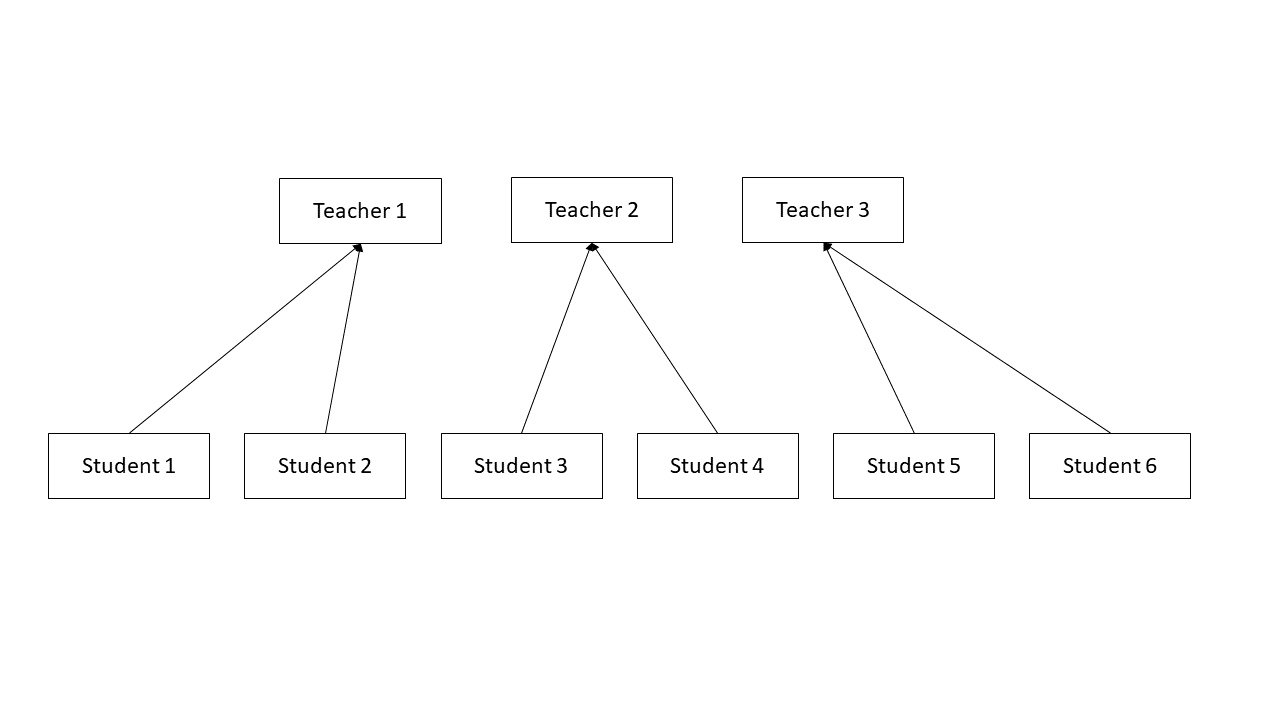
\includegraphics[width=17.78in]{Slide1} \caption{Figure 1: A pure hierarchical model}(\#fig:fig 1)
\end{figure}

\begin{table}

\caption{(\#tab:true hierarchical table)Data distribution indicating a true hierarchical model}
\centering
\begin{tabular}[t]{llll}
\toprule
student & Math\_Teacher\_1 & Math\_Teacher\_2 & Math\_Teacher\_3\\
\midrule
student & 1, 2 & 3, 4 & 5, 6\\
\bottomrule
\end{tabular}
\end{table}

Two level strict hierarchical models can be written as two separate equations, each representing a level of the model.\\
\[y_{ij} = \beta_{0j} + r_{ij}\]
\[\beta_{0j} = \gamma_{00} + u_{0j}\],

With these equations, \(y_{ij}\) is outcome and \(\beta_{0j}\) represents intercepts. In the intercept-only model presented, there are no slope components, but if we were to add in predictors, we could examine how slopes vary. \(r_{ij}\) is the random variation in level one, while \(u_{0j}\) is random variation in level 2 \citep{SnijdersICC}.

\hypertarget{non-hierarchical-models-in-brief}{%
\section{Non-hierarchical models in brief}\label{non-hierarchical-models-in-brief}}

While data can be purely hierarchical as described above, situations often arise when level 1 units do not fit neatly into one and only one level 2 cluster. One example of this type of non-hierarchical model is a cross-classified model. In this instance, level 1 units are members of more than one level two cluster, but there is not a pure hierarchy. For example, students may be nested within both biology classes and chemistry classes, with the outcome measurement being science knowledge. It would seem wise to take into account both the impact of biology classes as well as chemistry classes. However, students who were in the same biology class are not all in the same chemistry class. This situation would require the use of a cross-classified model. Cross-classified models, like pure hierarchical models, can also be represented in table or visual form. In table form, the cross classified structure becomes evident when there are level one units in more than one row and column. In the simple example below, there are multiple cells filled in both rows (Physics Teacher 1 and 2) and in columns (Math Teacher 2) \citep{Beretvas}.

\begin{figure}
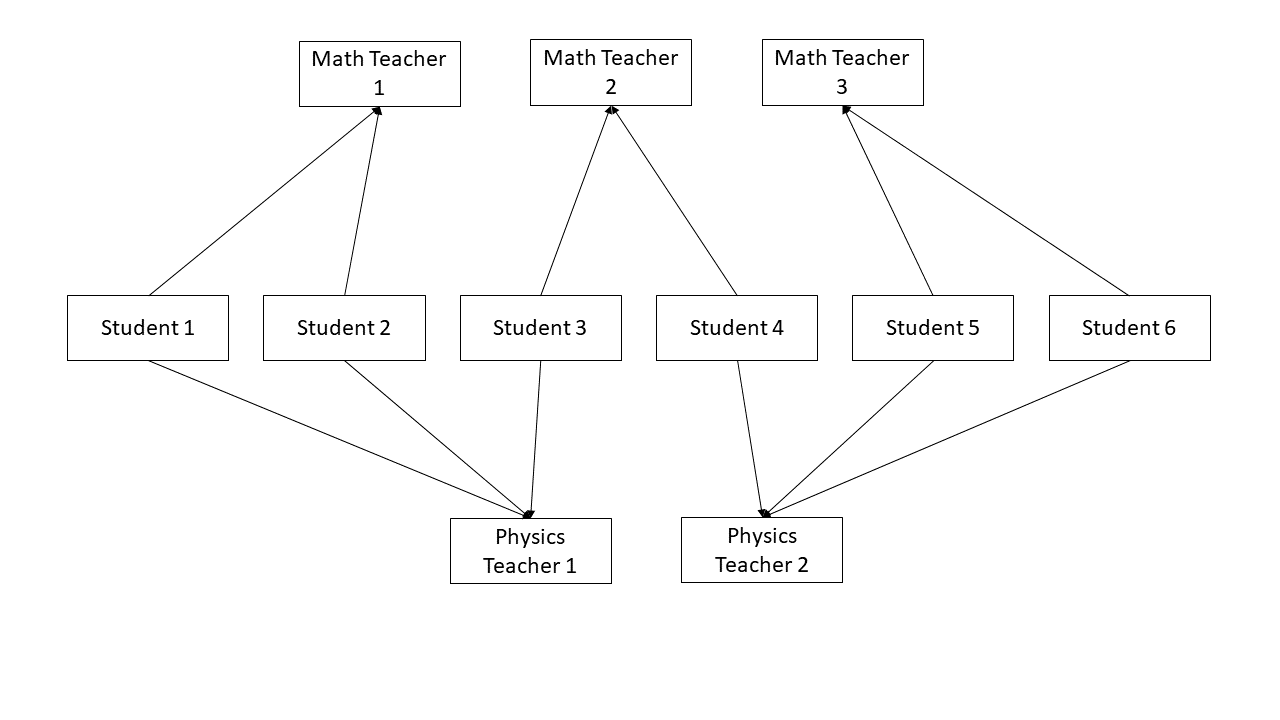
\includegraphics[width=17.78in]{Slide2} \caption{Figure 2: A Cross-classified model}(\#fig:fig 2)
\end{figure}

Another type of non-hierarchical model is a multiple membership model. In this instance, there is only one level 2 cluster being considered, but the level 1 units do not all belong to one and only one cluster. These types of models are frequently employed in education to model what are termed mobile students: students who attend more than one school over a given time frame. An example of mobile students might be those who attend more than one elementary school prior to a state-wide 5th grade test. Multiple membership data are also evident in table form, as well as in a unit diagram. As with the other diagrams, however, these can quickly become visually confusing with large data sets \citep[\citet{Beretvas}]{Leckie2013}.

\begin{figure}
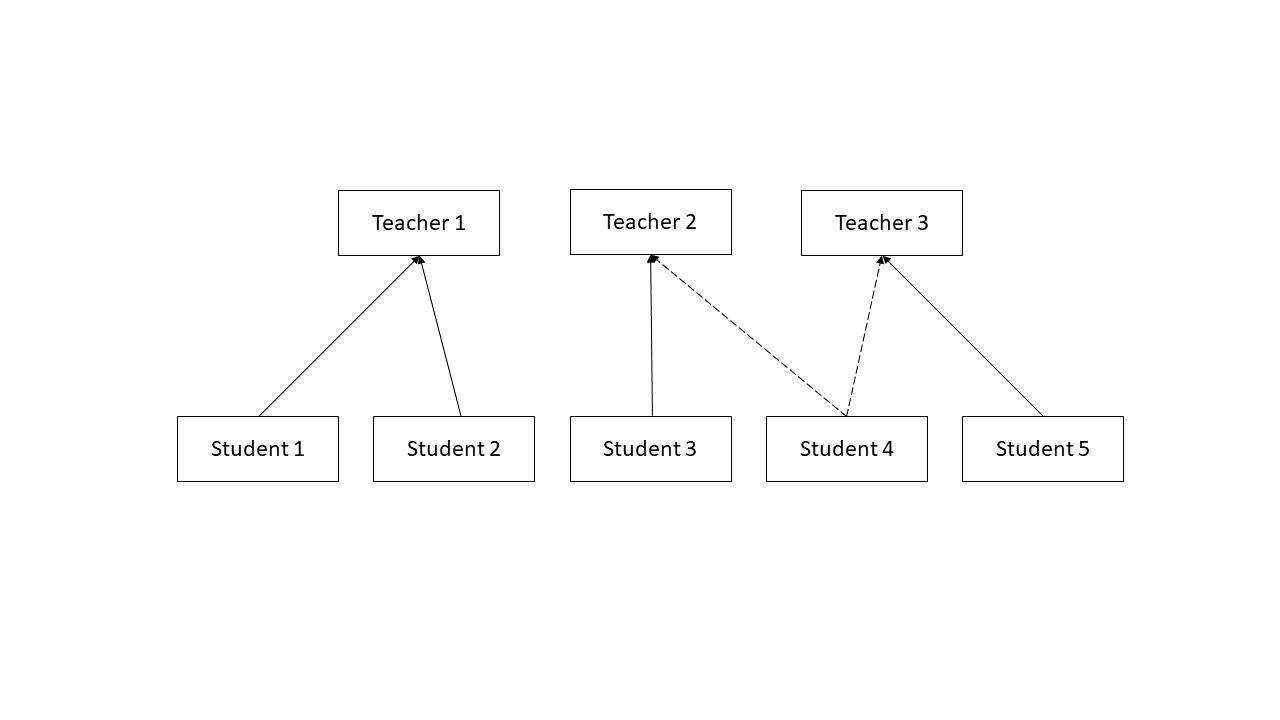
\includegraphics[width=17.78in]{Slide3} \caption{Figure 3: A Multiple Membership model}(\#fig:fig 3)
\end{figure}

Moving forward, we will focus exclusively on multiple membership models, going more in-depth into their intricacies as well as walking through a tutorial running a model and interpreting the output.

\hypertarget{data}{%
\chapter{Data}\label{data}}

The data used for this tutorial were simulated in R to loosely represent a cohort of JMU students. As accurate counts and frequencies of the predictors were not available outside of a request to PAIR, ``best guesses'' were employed where necessary. In a fictional scenario, JMU has decided to add a Math Achievement Test as a graduation requirement: students must take this test the semester they anticipate graduating as a measure of their Math Achievement at JMU, with the point of comparison being a cut-score. The stakes are similar to Assessment Day and there are no penalties for low scores. JMU, recognizing that many factors may play into how well a student does on this test, wants to consider the role different math teachers play as well as some student-level predictors. Not wanting this to hold any penalty towards teachers either, JMU has assigned each teacher an anonymous ID and associated it with the years of experience. JMU is additionally considering what teacher qualities help students be more successful, with the idea of offering more professional development in those areas. Currently, the only teacher-level predictor available is number of years of experience of the instructor.

JMU hopes to answer the following research questions:
RQ1: Do teacher characteristics influence student math scores?
RQ2: What student characteristics predict math scores?
RQ3: Does more teacher experience lead to better student outcomes?

The predictors are listed in the table below, along with a brief description.

\begin{table}

\caption{\label{tab:data}Simulated dataset that will be used for analysis}
\centering
\begin{tabular}[t]{ll}
\toprule
Predictor & Description\\
\midrule
MathAch & Mach Achievement; outcome variable, score on a (fictional) math test given to students\\
S\_ID & Student ID; a single number representation of students, from 1 to 5200\\
SAT\_M & SAT math score; ranges from 200-800 and represents the SAT math score of students prior to entering JMU.\\
S\_gend & Student gender; a non-binary gender indicator with 0 = female, 1 = male, and 2 = other/nonbinary/fluid\\
female, NB & Dummy coded student gender, since gender is categorical.  Male is the reference\\
\addlinespace
S\_SES & Student SES; values range from 2-29\\
num\_tchrs & Number of teachers; the number of math teachers a student had at JMU\\
phys & Physics; if a student took physics or not, with 0 = no and 1 = yes\\
phys\_tchr & Physics teacher; if a student took physics, the ID of the teacher they had (ranging from 1 – 22)\\
tchr1-tchr12 & Teachers 1 through 12; teacher IDs (ranging from 1-56) of teachers students had.  If a student had less than 12 teachers, teacher ID = 0\\
\addlinespace
w1-w12 & Weights; these represent the amount of time spent with each teacher.  Values can range from 1 (only had one teacher) to 0.083 (had 12 teachers)\\
t1\_exp-t12\_exp & Teacher experience; Given the compact nature of this dataset, the experience of the first through twelfth teachers of each student is given in years.\\
\bottomrule
\end{tabular}
\end{table}

\hypertarget{compact}{%
\section{Compact vs.~wide forms}\label{compact}}

The data are in a .cvs file in ``compact'' form, as opposed to ``wide'' form. Compact form contains two different sets of variables: one set for the first through twelfth teacher to instruct each student and another set represent the multiple membership weight variables. Wide form would have the same information, but in only one set of variables representing the individual teacher IDs and the proportion of time each teacher spent instructing each student in the cells (see tables below).

\hypertarget{compact-1}{%
\subsection{Compact}\label{compact-1}}

In compact form, there is a set of variables for the max number of level 2 units encountered, and another set of variables for the weights. Adding in a level-2 predictor here would only necessitate adding in the appropriate number of columns for the number of level 2 units encountered for that predictor. Using our data as an example, we have teacher experience as a level 2 predictor, and 12 possible teacher encounters. To add in teacher experience, we would add in 12 columns, t\_exp1-t\_exp12, which would populate with the appropriate experience for the teacher the student had. The weight would be calculated via the weight columns.

\begin{table}

\caption{(\#tab:compact ex)Data in compact form}
\centering
\begin{tabular}[t]{rrrrrrr}
\toprule
Student & Teacher.1 & Teacher.2 & Teacher.3 & w1 & w2 & w3\\
\midrule
1 & 2 & 4 & 1 & 0.33 & 0.33 & 0.33\\
2 & 2 & 3 & 1 & 0.33 & 0.33 & 0.33\\
3 & 3 & 1 & 4 & 0.33 & 0.33 & 0.33\\
4 & 0 & 3 & 0 & 0.00 & 1.00 & 0.00\\
5 & 1 & 0 & 0 & 1.00 & 0.00 & 0.00\\
\addlinespace
6 & 0 & 1 & 3 & 0.00 & 0.50 & 0.50\\
7 & 0 & 1 & 2 & 0.00 & 0.50 & 0.50\\
8 & 0 & 0 & 1 & 0.00 & 0.00 & 1.00\\
9 & 1 & 2 & 0 & 0.50 & 0.50 & 0.00\\
10 & 4 & 0 & 2 & 0.50 & 0.00 & 0.50\\
\bottomrule
\end{tabular}
\end{table}

\hypertarget{wide}{%
\subsection{Wide}\label{wide}}

While perhaps less evident in this small example, if there were more teacher IDs (56, as in our data for example), but a small number of level 2 units encountered and the associated weights (12 of each in our data), the `wide' descriptor would become more evident. The wide descriptor becomes even more evident when considering level two predictors in the model. In the wide format, every level-2 predictor we add will be calculated across all the level-2 ids. Using our data as an example, we have teacher experience as a level-2 predictor. Adding it in using a wide format would mean including 56 columns for the teacher IDs, with weights in the cell to represent the time each student spent with that teacher. Then, there would be another 56 columns for the teacher experience for each of the teachers, with each of their respective experiences.

\begin{table}

\caption{(\#tab:wide ex)Data in wide form}
\centering
\begin{tabular}[t]{rrrrr}
\toprule
Student & T1 & T2 & T3 & T4\\
\midrule
1 & 0.33 & 0.33 & 0.00 & 0.33\\
2 & 0.33 & 0.33 & 0.33 & 0.00\\
3 & 0.33 & 0.00 & 0.33 & 0.33\\
4 & 0.00 & 0.00 & 1.00 & 0.00\\
5 & 1.00 & 0.00 & 0.00 & 0.00\\
\addlinespace
6 & 0.50 & 0.00 & 0.50 & 0.00\\
7 & 0.50 & 0.50 & 0.00 & 0.00\\
8 & 1.00 & 0.00 & 0.00 & 0.00\\
9 & 0.50 & 0.50 & 0.00 & 0.00\\
10 & 0.00 & 0.50 & 0.00 & 0.50\\
\bottomrule
\end{tabular}
\end{table}

While the wide form is less efficient, some programs require the data to be in one form or the other. In this instance, MLwiN using Bayesian routines (what we will be using) requires compact form \citep{Leckie2013}.

\hypertarget{examining-the-data}{%
\section{Examining the Data}\label{examining-the-data}}

The next step is to determine what type of predictors we have and what they look like, as well as if we have a true hierarchical model, a ``nesting as nuisance'' model, or a non-hierarchical model such as cross-classified or multiple membership models. We will be looking for if students (in this case) belong to one and only one cluster (teachers), which would indicate a hierarchical approach or perhaps a ``nesting as nuisance'' approach. However, if, as is the case, students belong to multiple clusters, we will be taking a non-hierarchical approach. For this example, we are only considering one cluster, so we will be using a multiple membership design. We can see in the \texttt{num\_tchrs} column there are students ranging from having had 1 teacher to 12 teachers, indicating we have a multiple membership column. We could also look at the \texttt{tchr1} through \texttt{tchr12} columns, and see there are values in more than one of those - indicating that students have encountered more than one math teacher.

\begin{Shaded}
\begin{Highlighting}[]
\CommentTok{\#Read in the data file}
\NormalTok{StudData }\OtherTok{\textless{}{-}} \FunctionTok{read.csv}\NormalTok{(}\StringTok{"exampledata2.csv"}\NormalTok{)}

\CommentTok{\#See what it looks like}
\FunctionTok{head}\NormalTok{(StudData)}
\end{Highlighting}
\end{Shaded}

\begin{verbatim}
##   X.2 X.1 X S_ID S_gend     S_SES num_tchrs phys tchr1 tchr2 tchr3 tchr4 tchr5 tchr6 tchr7 tchr8 tchr9 tchr10 tchr11 tchr12   w1   w2   w3   w4 w5 w6 w7 w8 w9 w10 w11 w12
## 1   1   1 1    1      0 14.880674         3    0    24    32    46     0     0     0     0     0     0      0      0      0 0.33 0.33 0.33 0.00  0  0  0  0  0   0   0   0
## 2   2   2 2    2      0 14.575710         4    0    30    52    54    18     0     0     0     0     0      0      0      0 0.25 0.25 0.25 0.25  0  0  0  0  0   0   0   0
## 3   3   3 3    3      1 13.173884         1    0    12     0     0     0     0     0     0     0     0      0      0      0 1.00 0.00 0.00 0.00  0  0  0  0  0   0   0   0
## 4   4   4 4    4      1 13.065602         2    0    32    30     0     0     0     0     0     0     0      0      0      0 0.50 0.50 0.00 0.00  0  0  0  0  0   0   0   0
## 5   5   5 5    5      0 16.105715         2    0     3    48     0     0     0     0     0     0     0      0      0      0 0.50 0.50 0.00 0.00  0  0  0  0  0   0   0   0
## 6   6   6 6    6      1  8.190244         2    1     3    44     0     0     0     0     0     0     0      0      0      0 0.50 0.50 0.00 0.00  0  0  0  0  0   0   0   0
##       Math t10_exp    t1_exp    t2_exp   t3_exp   t4_exp t5_exp t6_exp t7_exp t8_exp t9_exp t11_exp t12_exp phys_tchr SAT_M female NB
## 1 530.3671       0  9.512710  9.603359 11.08068 0.000000      0      0      0      0      0       0       0         0   795      1  0
## 2 523.2353       0 10.138500 12.664019 11.33673 4.434515      0      0      0      0      0       0       0         0   693      1  0
## 3 457.6296       0 12.682655  0.000000  0.00000 0.000000      0      0      0      0      0       0       0         0   706      0  0
## 4 504.4141       0  9.603359 10.138500  0.00000 0.000000      0      0      0      0      0       0       0         0   654      0  0
## 5 443.2032       0  9.541097 12.631969  0.00000 0.000000      0      0      0      0      0       0       0         0   419      1  0
## 6 431.5336       0  9.541097 11.309230  0.00000 0.000000      0      0      0      0      0       0       0         9   416      0  0
\end{verbatim}

\begin{Shaded}
\begin{Highlighting}[]
\FunctionTok{summary}\NormalTok{(StudData)}
\end{Highlighting}
\end{Shaded}

\begin{verbatim}
##       X.2            X.1             X             S_ID          S_gend           S_SES          num_tchrs           phys            tchr1           tchr2           tchr3       
##  Min.   :   1   Min.   :   1   Min.   :   1   Min.   :   1   Min.   :0.0000   Min.   : 5.657   Min.   : 1.000   Min.   :0.0000   Min.   : 1.00   Min.   : 0.00   Min.   : 0.000  
##  1st Qu.:1301   1st Qu.:1301   1st Qu.:1301   1st Qu.:1301   1st Qu.:0.0000   1st Qu.:11.652   1st Qu.: 1.000   1st Qu.:0.0000   1st Qu.:14.00   1st Qu.: 0.00   1st Qu.: 0.000  
##  Median :2600   Median :2600   Median :2600   Median :2600   Median :0.0000   Median :12.988   Median : 2.000   Median :0.0000   Median :29.00   Median :14.00   Median : 0.000  
##  Mean   :2600   Mean   :2600   Mean   :2600   Mean   :2600   Mean   :0.4708   Mean   :12.996   Mean   : 2.593   Mean   :0.2492   Mean   :28.61   Mean   :18.73   Mean   : 9.415  
##  3rd Qu.:3900   3rd Qu.:3900   3rd Qu.:3900   3rd Qu.:3900   3rd Qu.:1.0000   3rd Qu.:14.353   3rd Qu.: 4.000   3rd Qu.:0.0000   3rd Qu.:43.00   3rd Qu.:35.00   3rd Qu.:14.000  
##  Max.   :5200   Max.   :5200   Max.   :5200   Max.   :5200   Max.   :2.0000   Max.   :20.249   Max.   :12.000   Max.   :1.0000   Max.   :56.00   Max.   :57.00   Max.   :57.000  
##      tchr4            tchr5           tchr6            tchr7             tchr8             tchr9             tchr10            tchr11            tchr12              w1        
##  Min.   : 0.000   Min.   : 0.00   Min.   : 0.000   Min.   : 0.0000   Min.   : 0.0000   Min.   : 0.0000   Min.   : 0.0000   Min.   : 0.0000   Min.   : 0.0000   Min.   :0.0830  
##  1st Qu.: 0.000   1st Qu.: 0.00   1st Qu.: 0.000   1st Qu.: 0.0000   1st Qu.: 0.0000   1st Qu.: 0.0000   1st Qu.: 0.0000   1st Qu.: 0.0000   1st Qu.: 0.0000   1st Qu.:0.2500  
##  Median : 0.000   Median : 0.00   Median : 0.000   Median : 0.0000   Median : 0.0000   Median : 0.0000   Median : 0.0000   Median : 0.0000   Median : 0.0000   Median :0.5000  
##  Mean   : 7.238   Mean   : 5.06   Mean   : 2.625   Mean   : 0.4515   Mean   : 0.4065   Mean   : 0.3956   Mean   : 0.3735   Mean   : 0.3406   Mean   : 0.2996   Mean   :0.5784  
##  3rd Qu.: 1.000   3rd Qu.: 0.00   3rd Qu.: 0.000   3rd Qu.: 0.0000   3rd Qu.: 0.0000   3rd Qu.: 0.0000   3rd Qu.: 0.0000   3rd Qu.: 0.0000   3rd Qu.: 0.0000   3rd Qu.:1.0000  
##  Max.   :57.000   Max.   :56.00   Max.   :57.000   Max.   :55.0000   Max.   :56.0000   Max.   :56.0000   Max.   :56.0000   Max.   :57.0000   Max.   :57.0000   Max.   :1.0000  
##        w2               w3                w4                w5                w6                w7                 w8                w9               w10          
##  Min.   :0.0000   Min.   :0.00000   Min.   :0.00000   Min.   :0.00000   Min.   :0.00000   Min.   :0.000000   Min.   :0.00000   Min.   :0.00000   Min.   :0.000000  
##  1st Qu.:0.0000   1st Qu.:0.00000   1st Qu.:0.00000   1st Qu.:0.00000   1st Qu.:0.00000   1st Qu.:0.000000   1st Qu.:0.00000   1st Qu.:0.00000   1st Qu.:0.000000  
##  Median :0.2000   Median :0.00000   Median :0.00000   Median :0.00000   Median :0.00000   Median :0.000000   Median :0.00000   Median :0.00000   Median :0.000000  
##  Mean   :0.2424   Mean   :0.07666   Mean   :0.04988   Mean   :0.03008   Mean   :0.01458   Mean   :0.001487   Mean   :0.00124   Mean   :0.00112   Mean   :0.001035  
##  3rd Qu.:0.5000   3rd Qu.:0.16600   3rd Qu.:0.08300   3rd Qu.:0.00000   3rd Qu.:0.00000   3rd Qu.:0.000000   3rd Qu.:0.00000   3rd Qu.:0.00000   3rd Qu.:0.000000  
##  Max.   :0.5000   Max.   :0.33000   Max.   :0.25000   Max.   :0.20000   Max.   :0.16600   Max.   :0.142800   Max.   :0.12500   Max.   :0.11000   Max.   :0.100000  
##       w11                 w12                 Math          t10_exp            t1_exp           t2_exp           t3_exp           t4_exp           t5_exp           t6_exp       
##  Min.   :0.0000000   Min.   :0.0000000   Min.   :283.9   Min.   : 0.0000   Min.   : 4.435   Min.   : 0.000   Min.   : 0.000   Min.   : 0.000   Min.   : 0.000   Min.   : 0.0000  
##  1st Qu.:0.0000000   1st Qu.:0.0000000   1st Qu.:396.6   1st Qu.: 0.0000   1st Qu.: 9.300   1st Qu.: 0.000   1st Qu.: 0.000   1st Qu.: 0.000   1st Qu.: 0.000   1st Qu.: 0.0000  
##  Median :0.0000000   Median :0.0000000   Median :442.4   Median : 0.0000   Median :10.725   Median : 9.112   Median : 0.000   Median : 0.000   Median : 0.000   Median : 0.0000  
##  Mean   :0.0009777   Mean   :0.0009258   Mean   :442.0   Mean   : 0.1229   Mean   :10.453   Mean   : 6.928   Mean   : 3.449   Mean   : 2.618   Mean   : 1.806   Mean   : 0.9881  
##  3rd Qu.:0.0000000   3rd Qu.:0.0000000   3rd Qu.:486.1   3rd Qu.: 0.0000   3rd Qu.:11.512   3rd Qu.:11.126   3rd Qu.: 9.112   3rd Qu.: 4.435   3rd Qu.: 0.000   3rd Qu.: 0.0000  
##  Max.   :0.0900000   Max.   :0.0830000   Max.   :614.1   Max.   :14.0426   Max.   :14.728   Max.   :14.728   Max.   :14.728   Max.   :14.728   Max.   :14.728   Max.   :14.7281  
##      t7_exp            t8_exp            t9_exp           t11_exp           t12_exp          phys_tchr         SAT_M           female             NB        
##  Min.   : 0.0000   Min.   : 0.0000   Min.   : 0.0000   Min.   : 0.0000   Min.   : 0.0000   Min.   : 0.00   Min.   :200.0   Min.   :0.0000   Min.   :0.0000  
##  1st Qu.: 0.0000   1st Qu.: 0.0000   1st Qu.: 0.0000   1st Qu.: 0.0000   1st Qu.: 0.0000   1st Qu.: 0.00   1st Qu.:350.0   1st Qu.:0.0000   1st Qu.:0.0000  
##  Median : 0.0000   Median : 0.0000   Median : 0.0000   Median : 0.0000   Median : 0.0000   Median : 0.00   Median :500.0   Median :1.0000   Median :0.0000  
##  Mean   : 0.1677   Mean   : 0.1475   Mean   : 0.1378   Mean   : 0.1203   Mean   : 0.1151   Mean   : 2.88   Mean   :499.8   Mean   :0.5717   Mean   :0.0425  
##  3rd Qu.: 0.0000   3rd Qu.: 0.0000   3rd Qu.: 0.0000   3rd Qu.: 0.0000   3rd Qu.: 0.0000   3rd Qu.: 0.00   3rd Qu.:646.2   3rd Qu.:1.0000   3rd Qu.:0.0000  
##  Max.   :14.7281   Max.   :13.9805   Max.   :14.7281   Max.   :14.7281   Max.   :14.7281   Max.   :22.00   Max.   :800.0   Max.   :1.0000   Max.   :1.0000
\end{verbatim}

We can also see distributions of the outcome and predictors.
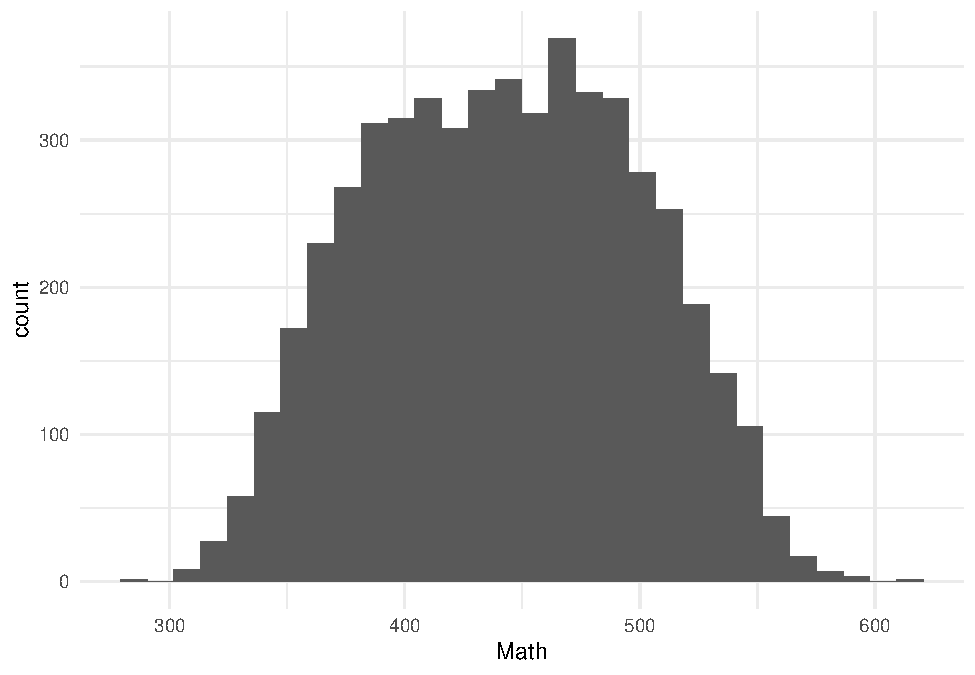
\includegraphics{_main_files/figure-latex/outcome-1.pdf}
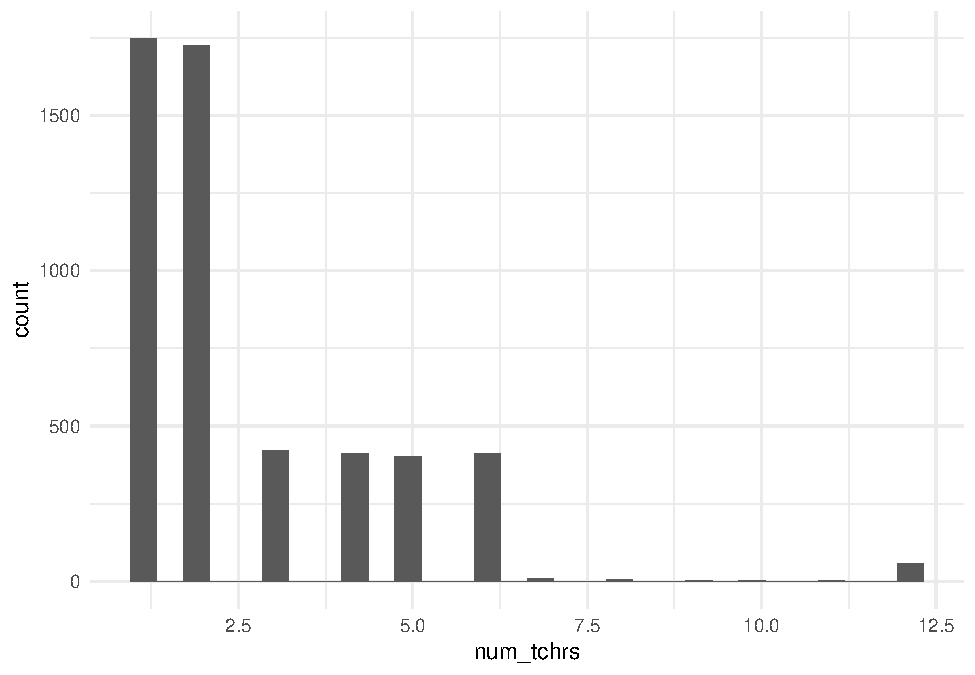
\includegraphics{_main_files/figure-latex/predictors1-1.pdf}
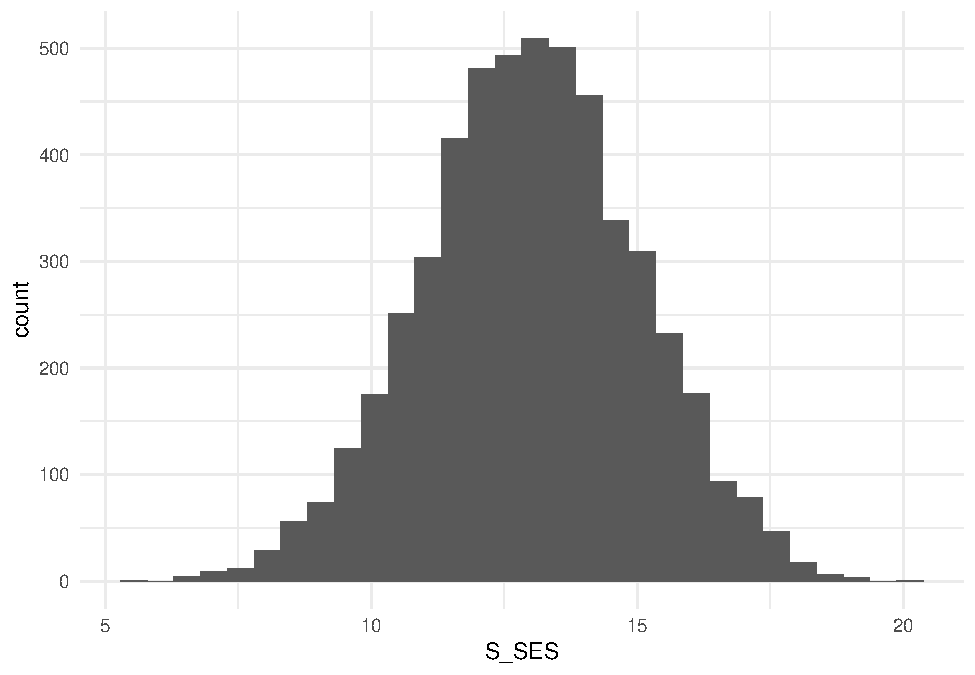
\includegraphics{_main_files/figure-latex/predictors2-1.pdf}
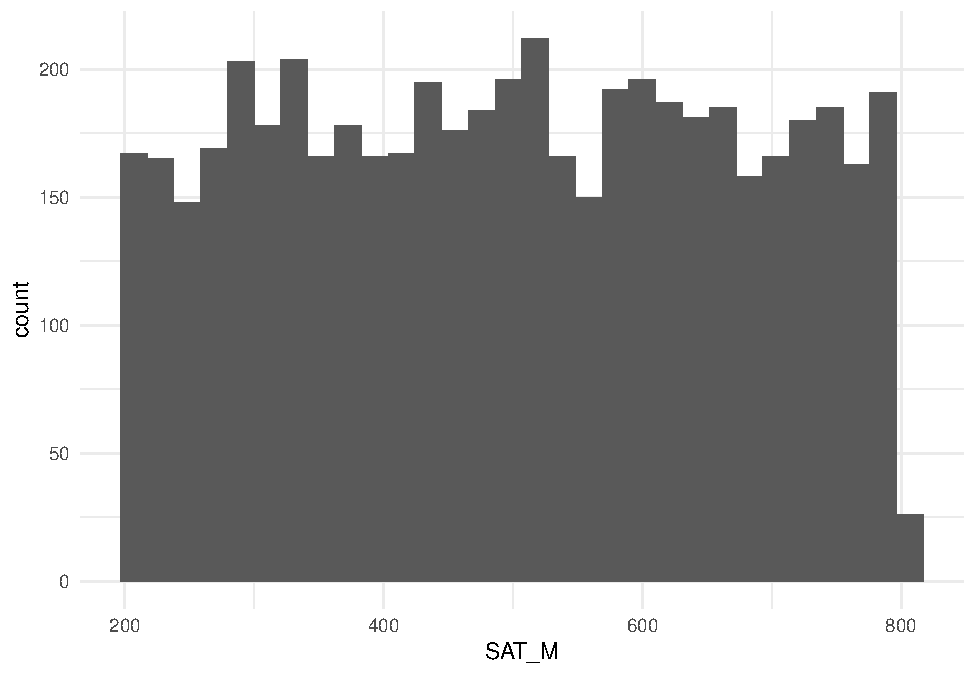
\includegraphics{_main_files/figure-latex/predictors3-1.pdf}

\hypertarget{software}{%
\section{Software Considerations}\label{software}}

MLwiN\citep{MLwiN} is one of the most commonly found software programs for running multiple membership models, as it can natively handle such complex models. I have found that SAS and Stata can be `tricked' into running simple multiple membership models by fitting them as constrained hierarchical models, but with non-continuous outcomes or increased complexity they quickly become computationally inefficient. More worryingly is that the parameter estimates generated by these methods are found to be biased. The same sources say that R can also be tricked, but I have not found that to be the case \citep{Stata2013}. That said, both R and Stata have functions or packages that allow you to use their interface and run MLwiN in the background, both to allow use of a familiar interface but also to allow for accurate estimation methods with full model recognition. MLwiN is not a free software and is produced by the University of Bristol. A 30-day free trial with full functionality is available to anyone in the world, and for researchers in the US, a single-user license is £400 or a PhD license is available for £225, though it expires after 3 years. In order to perform the analyses demonstrated below, I obtained a 30-day free license and used the R2MLwiN \citep{R-R2MLwiN} package to allow me to use an R interface. While the R code is provided, it will not work unless you also have a valid MLwiN license.

\citet{Heck2022} used OpenBUGS for some more complex multiple membership cross classified modeling of longitudinal data, but at this time OpenBUGS website no longer exists and has been ported to MultiBUGS \citep[\citet{BUGS2020}]{MultiBUGS}. One potential drawback of this program is the mis-classification of its software framework by virus detection programs as a virus, leading it to be uninstallable or to throw errors. MultiBUGS also reports that an R interface (R2MultiBUGS) is under development.

\hypertarget{multiple-membership-models-the-details}{%
\chapter{Multiple Membership models: the details}\label{multiple-membership-models-the-details}}

The key feature of a multiple membership model is that level 1 units do not belong to one and only one level 2 cluster. There may be some units that exhibit true hierarchy, but there are others that are `multiple members': they belong to 2 or more clusters. A classic example of this is mobile students in educational settings (eg. \citet{Chung2012}, \citet{Heck2022}, \citet{Leroux}). Another example in the health care setting is patient outcomes, but each patient frequently sees more than one nurse \citep{Leckie2013}. Using a multiple membership model allows the influence of multiple level 2 clusters to be taken into account. Additionally, just like ignoring hierarchical data violates the independent observations assumption and cause an inflated type I error rate, ignoring a multiple membership structure of your data will also cause an inflated type I error rate.

Historically, when researchers encountered a multiple membership data structure (ie, mobile students) and were unable to model it correctly, there were a few options to handle this data that they would choose from, all of which resulted in mis-specified models. In one option, researchers would only consider the unit to be a member of their most recent cluster. As an example, only consider the school a child was in at the time of testing, rather than any other previous schools. Another option was to simply delete the mobile students from the data set, leaving only a pure hierarchy of students nested in schools. A third option was to acknowledge the mobility of students by including a dichotomous or ordinal ``mobility'' predictor to include in a regular hierarchical model. This would control for the influence of mobility on the outcome, but did not allow for the modeling of the effects of different schools on the student. However, none of these methods are an appropriate treatment of multiple membership data. The results obtained from the `delete mobile students' approach, for example, can only be generalized to other non-mobile students as well as decreasing the power. In the study by \citet{Chung2012}, they reported negative bias in the level 2 predictor coefficients and in the level 2 variance components when employing the `only count the last school' technique. In the same study, they also found that the level 1 variance components were positively biased. It is for these reasons that researchers investigating multiple membership data use a multiple membership model, in order to allow for generalization of results, proper capturing of mobile student effects, and validity of inferences about school effects \citep{Smith2017}.

\hypertarget{notation}{%
\section{Notation}\label{notation}}

There are three possibilities for how to depict these models, each with its own set of advantages and disadvantages. Standard hierarchical notation, which we are familiar with from truly hierarchical models, uses subscripts to identify individual and cluster level predictors and effects. The disadvantage of this notation is that, due to its familiarity, individuals may incorrectly assume that unit \(\textit{i}\) is strictly nested within cluster \(\textit{j}\), which is not the case (\citet{SnijdersICC}; \citet{Leckie2013}). Another method is to use multiple subscript notation (\citet{Beretvas}). This notation makes the non-hierarchical structure more apparent, however, it can quickly become challenging to read.

The notation we will use moving forward is classification notation \citep{Leckie2013}:\\
\[y_{i} = \beta_{0} + \sum_{j \in school(i)}w_{j,i}^{(2)}u_{j}^{(2)} + e_{i}\]
\[u_{j}^{(2)} \sim N(0, \sigma_{u(2)}^{2})\]
\[e_{i} \sim N(0, \sigma_{e}^{2})\]
With this notation, the multiple membership component is represented by \(\sum_{j \in school(i)}w_{j,i}^{(2)}u_{j}^{(2)}\), which represents the weighted (\(w_{j,i}^{(2)}\)) cluster effects (\(u_{j}^{(2)}\)). The weight component represents the amount of time unit \(\textit{i}\) spent in cluster \(\textit{j}\), with the superscript (2) representing this is associated with the second level. All levels in the model are indicated, with level 1 (1) being implicit. The superscripts/subscripts for each level will identify to which level the random effects, variance parameters, and covariance parameters are associated with.

\hypertarget{weights}{%
\section{Weights}\label{weights}}

Weights are assigned to the level two clusters to reflect the different influences each one has on the level 1 units, and sum to one for any given level 1 unit. These are decided by the researcher, who may take one of several approaches. One approach is to assign equal weights, regardless of time. This is the approach taken in the example data set for this tutorial: it was assumed that each teacher seen by a student had equal influence, and the data set was designed in such a way that students did not see any given teacher more than once. In a mobile student situation, it may be that if a student attended a school for any length of time, that school would be given an equal weight to all the other schools attended by the student, even if they attended other schools for longer. Another approach is to account for length of time. In the previous example, if a student spent 1 year at school 1 but 2 years at school two, a researcher may weight school one as 0.33 and school 2 as 0.67. This will take into account the fact that since the student spent more time at school 2, it likely had a larger impact. A third approach seen is weighting later educational settings more heavily than earlier ones, to reflect the fact that the more recent education may have a larger impact on test scores (for example) than earlier education \citep{Chung2012}.

If we look at the data (\ref@data), we can pull two students to see the earlier equation written out for each of them, student 1 and student 3. For student 1, we see that they had three teachers (24, 32, and 46) while student 3 only had one teacher (12). The equations for students 3 and 1 are shown below, indicating the role cluster weights play in these models.

\hypertarget{student-3}{%
\subsection{Student 3}\label{student-3}}

\[y_{3} = \beta_{0} + \sum_{j \in \{12\}}w_{j,3}^{(2)}u_{j}^{(2)} + e_{3}\]\\
\[ = \beta_{0} + w_{12,3}^{(2)}u_{12}^{(2)} + e_{3}\]\\
\[ = \beta_{0} + u_{12}^{(2)} + e_{3}\]

\hypertarget{student-1}{%
\subsection{Student 1}\label{student-1}}

\[y_{1} = \beta_{0} + \sum_{j \in \{24, 32, 46\}}w_{j,1}^{(2)}u_{j}^{(2)} + e_{1}\]\\
\[ = \beta_{0} + w_{24,1}^{(2)}u_{24}^{(2)} + w_{32,1}^{(2)}u_{32}^{(2)} + w_{46,1}^{(2)}u_{46}^{(2)}+ e_{1}\]\\
\[ = \beta_{0} + 0.33u_{24}^{(2)} + 0.33u_{32}^{(2)} + 0.33u_{46}^{(2)}+ e_{1}\]

These weights are used both to identify amount of belonging to a particular level 2 cluster, but also to appropriately weight any level 2 predictors. For example, if we were to add in \texttt{t\_exp} as teacher-level predictor, the resulting equations would look like this:

\[y_{i} = \beta_{0} + \beta_{1}\sum_{j \in school(i)}w_{j,i}^{(2)}t\_exp_{2j}^{(2)} + \sum_{j \in school(i)}w_{j,i}^{(2)}u_{j}^{(2)} + e_{i}\]
\[u_{j}^{(2)} \sim N(0, \sigma_{u(2)}^{2})\]
\[e_{i} \sim N(0, \sigma_{e}^{2})\]

The term \(\sum_{j \in school(i)}w_{j,i}^{(2)}t\_exp_{2j}^{(2)}\) is teacher experience (\texttt{t\_exp}), taking into account that since students saw different teachers, the experience of those teachers will be different. This is called the weighted sum of this predictor, with \(\beta_{1}\) being the slope coefficient. We are able to keep the term as-is in our equation, or to simplify the equation, we could calculate it in our data set to be \(\bar x_{2i}\). The resulting equation would then be

\[y_{i} = \beta_{0} + \beta_{1}\overline{(t\_exp)}_{2i} + \sum_{j \in school(i)}w_{j,i}^{(2)}u_{j}^{(2)} + e_{i}\]

\hypertarget{centering}{%
\section{Centering}\label{centering}}

In pure hierarchical models, predictors (typically at level 1) can either be group mean centered (CWC) or grand mean centered (CGM), with CWC being the generally preferred option due to the resulting interpretability of the coefficients \citep{Enders2013}. However, in a multiple membership model, level 1 units belong to one or more level 2 clusters, meaning group mean centering can get really complicated really fast and indeed may not be possible. If centering is mentioned in the literature surrounding multiple membership models, it is only grand mean centering that is referenced. This may be due to ease, or due to lack of exploration using group mean centering. It may also be due to requiring a large sample size to have enough units in each unique `cluster' combination. For example, students who just had teacher 1 would be a cluster, while students who had teacher 1 and teacher 2 would be another cluster, etc. In our example with 56 teachers, and a max draw of 12 teachers, there are slightly more combinations than our sample size by several orders of magnitude. Much of the literature using multiple membership models (eg. \citep[\citet{Heck2022}, \citet{Ma2021}, \citet{Gero2020}]{Leckie2013}) did not mention any type of centering; an example where it was mentioned is \citet{Smith2017}, where grand mean centering is specifically addressed in their model descriptions.

\hypertarget{vpc-and-icc}{%
\section{VPC and ICC}\label{vpc-and-icc}}

\hypertarget{icc}{%
\subsection{ICC}\label{icc}}

Again comparing to pure hierarchical models, one of the first things that is calculated after running an intercept-only model is the ICC, or intraclass correlation. When calculated as \(\frac{\tau_{00}}{\tau_{00} + \sigma^{2}}\), the ICC represents the amount of variance in the outcome variable that can be attributed to the fact that level 1 units are nested in level 2 clusters \citep{SnijdersICC}. As with most things thus far, calculating an ICC for a multiple membership model is not so straightforward. The equation for a multiple membership model is more complex, and takes into account the cluster `profile' of two units. If we are looking at the cluster level ICC for two different units, \(\textit{i}\) and \(\textit{i'}\), we would calculate it as a correlation like so:
\[corr(y_{i}, y_{i'}) = \frac{\sigma_{u(2)}^{2}\sum_{j \in cluster(i) \cup cluster(i')}w_{j,i}^{(2)}w_{j, i'}^{(2)}}{\sqrt{\sigma_{u(2)}^{2}\sum_{j \in cluster(i)}w_{j,i}^{(2)} + \sigma_{e}^2}\sqrt{\sigma_{u(2)}^{2}\sum_{j \in cluster(i')}w_{j,i'}^{(2)} + \sigma_{e}^2}}\]

Interpreting the ICC as the correlation between the outcomes of two students who had the same teacher, and only that teacher, it would be calculated as
\[ICC = \frac{\sigma_{u(2)}^{2}}{\sigma_{u(2)}^{2} + \sigma_{e}^{2}}\]
However, if these students had two teachers each, and only shared one of them, the calculation for the ICC becomes
\[ICC = \frac{0.25\sigma_{u(2)}^{2}}{0.5\sigma_{u(2)}^{2} + \sigma_{e}^{2}}\]
This is because the weights for each teacher are incorporated to reflect the amount of time two students had similar teachers and the amount of time they had different teachers \citep{Leckie2013}.

\hypertarget{vpc}{%
\subsection{VPC}\label{vpc}}

Another way to determine how variance is partitioned in a model is the variance partition coefficient. This reports the proportion of observed variation in the outcome that is at each level. The VPC is different from the ICC in that it is not the model implied correlation within a cluster, but the observed variation. As with the ICC, the multiple membership model is more complex in this calculation as well. The variation in outcomes that can be attributed to clusters depends on how much the level 1 units are spread across clusters: are they members of one cluster or multiple clusters? The cluster-level VPC equation representing the amount of variation in outcomes that is attributed to clusters in a multiple membership model is \citep{Leckie2013}
\[VPC_{u(2)} = \frac{\sigma_{u(2)}^{2}\sum_{j \in cluster(i)}(w_{j,i}^{(2)})^2}{\sigma_{u(2)}^{2}\sum_{j \in cluster(i)}(w_{j,i}^{(2)})^2 + \sigma_{e}^{2}}\]

If we consider the level 1 units that were members of only one cluster, the VPC is equivalent to the ICC for two individuals that had the same, single, teacher above:\\
\[VPC_{u(2)} = \frac{\sigma_{u(2)}^{2}}{\sigma_{u(2)}^{2} + \sigma_{e}^{2}}\]
As above, however, it gets more complex when level 1 units are members of more than one cluster, and it no longer equals the ICC. Following a similar pattern to above, if we consider the population of level 1 units that were members of two different clusters (which one is not important here; we are looking only at cluster-level variance), the VPC calculation becomes
\[VPC_{u(2)} = \frac{0.5\sigma_{u(2)}^{2}}{0.5\sigma_{u(2)}^{2} + \sigma_{e}^{2}}\]
What this illustrates is that as level 1 units are members of more clusters, the amount of variance in outcomes that is attributed to clusters decreases. Additionally, with a multiple membership model, this is perhaps the easier of the two to both compute and calculate, as we are not considering how the cluster pattern of two individuals compares but rather how many clusters an individual is a member of.

\hypertarget{running-a-multiple-membership-model}{%
\chapter{Running a Multiple Membership Model}\label{running-a-multiple-membership-model}}

As noted in \ref{software}, we will be using MLwiN to evaluate the multiple membership models. There is an R package, R2MLwiN \citep{R-R2MLwiN} that allows for an R-interface which runs MLwiN in the background. This allows users to work with a program they are already familiar with while accessing the capabilities of MLwiN. However, as also previously noted, you must have an active MLwiN license, and have the program installed on your computer for your R code to work.

\hypertarget{intercept-only-model}{%
\section{Intercept-only Model}\label{intercept-only-model}}

We will first run an intercept-only model, looking at Math as an outcome and only including the intercept and the multiple membership effect of teachers. This model will inform us as to how the variance in Math scores is divided between teacher variance components (level 2) and student variance components (level 1).\\
\[y_{i} = \beta_{0} + \sum_{j \in school(i)}w_{j,i}^{(2)}u_{j}^{(2)} + e_{i}\]
\[u_{j}^{(2)} \sim N(0, \sigma_{u(2)}^{2})\]
\[e_{i} \sim N(0, \sigma_{e}^{2})\]

\hypertarget{first-steps}{%
\subsection{First Steps}\label{first-steps}}

Setting this up to run in R, we first need to make sure we have MLwiN installed, as well as call the \texttt{R2MLwiN} package. Additionally, R2MLwiN defaults the path to MLwiN as ``C:/Program Files/MLwiN v3.06/''. If yours, like mine, is installed elsewhere, you need to include \texttt{options(MLwiN\_pah\ =\ "path/to/MLwiN")}. An easy way to copy the path is to find it in your computer, hold `shift' and right click the program. The option ``copy as path'' comes up as an option, and you can just paste it in.

\hypertarget{define-the-model}{%
\subsection{Define the model}\label{define-the-model}}

After we have loaded in the appropriate packages, we take a few steps to actually run the model. First, we define the intercept-only model, including both the teacher columns and the student IDs. For our dataset, our model definition will be \texttt{intonly\ \textless{}-\ Math\ \textasciitilde{}\ 1\ +\ (1\textbar{}tchr1)\ +\ (1\textbar{}S\_ID)}. Important to note is that when defining the teacher columns (\texttt{(1\textbar{}tchr1)}), we use the first column name, not \texttt{tchr} as you might be inclined to do. The random part of the model, \texttt{(1\textbar{}tchr1)} and \texttt{(1\textbar{}S\_ID)}, is written in descending order of hierarchy. With this model specification, we are allowing intercepts to vary at level 2 (\texttt{(1\textbar{}tchr1)}) and level 1 (\texttt{(1\textbar{}S\_ID)}).

\hypertarget{set-up-and-send-to-mlwin}{%
\subsection{Set up and send to MLwiN}\label{set-up-and-send-to-mlwin}}

The next step is to define the multiple membership variables (teacher columns for us) and the associated weights. To do this, we make an object that is a list of list of lists. I named it \texttt{MultiMemb} in the code chunk below:

\begin{Shaded}
\begin{Highlighting}[]
\NormalTok{MultiMemb }\OtherTok{\textless{}{-}} \FunctionTok{list}\NormalTok{(}\FunctionTok{list}\NormalTok{(}
  \AttributeTok{mmvar =} \FunctionTok{list}\NormalTok{(}\StringTok{"tchr1"}\NormalTok{, }\StringTok{"tchr2"}\NormalTok{, }\StringTok{"tchr3"}\NormalTok{, }\StringTok{"tchr4"}\NormalTok{, }\StringTok{"tchr5"}\NormalTok{, }\StringTok{"tchr6"}\NormalTok{, }\StringTok{"tchr7"}\NormalTok{, }\StringTok{"tchr8"}\NormalTok{, }\StringTok{"tchr9"}\NormalTok{, }\StringTok{"tchr10"}\NormalTok{, }\StringTok{"tchr11"}\NormalTok{, }\StringTok{"tchr12"}\NormalTok{),}
  \AttributeTok{weights =} \FunctionTok{list}\NormalTok{(}\StringTok{"w1"}\NormalTok{, }\StringTok{"w2"}\NormalTok{, }\StringTok{"w3"}\NormalTok{, }\StringTok{"w4"}\NormalTok{, }\StringTok{"w5"}\NormalTok{, }\StringTok{"w6"}\NormalTok{, }\StringTok{"w7"}\NormalTok{, }\StringTok{"w8"}\NormalTok{, }\StringTok{"w9"}\NormalTok{, }\StringTok{"w10"}\NormalTok{, }\StringTok{"w11"}\NormalTok{, }\StringTok{"w12"}\NormalTok{)), }\ConstantTok{NA}\NormalTok{)}
\end{Highlighting}
\end{Shaded}

Within this, \texttt{mmvar} specifies classification units (unit of multiple membership). \texttt{weights} is where the associated weights go, and is the student-level weighting (in our case) given to each teacher they had. The final \texttt{NA} indicates that level 1 has no multiple membership classification. This set-up is why our data needed to be in compact rather than long form (\ref{compact}).

After we have defined \texttt{MultiMemb}, we can actually run the model. This line is putting everything together:

\begin{Shaded}
\begin{Highlighting}[]
\NormalTok{(MMembModel1 }\OtherTok{\textless{}{-}} \FunctionTok{runMLwiN}\NormalTok{(}\AttributeTok{Formula =}\NormalTok{ intonly, }\AttributeTok{data =}\NormalTok{ StudData, }\AttributeTok{estoptions =} \FunctionTok{list}\NormalTok{(}\AttributeTok{EstM =} \DecValTok{1}\NormalTok{, }\AttributeTok{drop.data =} \ConstantTok{FALSE}\NormalTok{, }\AttributeTok{mm =}\NormalTok{ MultiMemb)))}
\end{Highlighting}
\end{Shaded}

Looking at it, we are calling MLwiN with \texttt{runMLwiN}, defining what the model should be with \texttt{Formula}, and defining our data set with \texttt{data}. \texttt{estoptions} is our estimation options. When \texttt{EstM} is equal to 1, we are using MCMC estimation. And lastly, within that same statement, \texttt{mm} is calling our \texttt{MultiMemb} object to match everything up and weight appropriately \citep{R-R2MLwiN}.

\hypertarget{put-it-all-together}{%
\subsection{Put it all together}\label{put-it-all-together}}

Taking everything from above and putting it all together, we get the following code chunk, and then output.

\begin{Shaded}
\begin{Highlighting}[]
\FunctionTok{library}\NormalTok{(R2MLwiN)}
\FunctionTok{options}\NormalTok{(}\AttributeTok{MLwiN\_path=}\StringTok{"C:}\SpecialCharTok{\textbackslash{}\textbackslash{}}\StringTok{Program Files (x86)}\SpecialCharTok{\textbackslash{}\textbackslash{}}\StringTok{MLwiN trial}\SpecialCharTok{\textbackslash{}\textbackslash{}}\StringTok{i386}\SpecialCharTok{\textbackslash{}\textbackslash{}}\StringTok{mlwin.exe"}\NormalTok{)}

\NormalTok{intonly }\OtherTok{\textless{}{-}}\NormalTok{ Math }\SpecialCharTok{\textasciitilde{}} \DecValTok{1} \SpecialCharTok{+}\NormalTok{ (}\DecValTok{1}\SpecialCharTok{|}\NormalTok{tchr1) }\SpecialCharTok{+}\NormalTok{ (}\DecValTok{1}\SpecialCharTok{|}\NormalTok{S\_ID)}

\NormalTok{MultiMemb }\OtherTok{\textless{}{-}} \FunctionTok{list}\NormalTok{(}\FunctionTok{list}\NormalTok{(}
  \AttributeTok{mmvar =} \FunctionTok{list}\NormalTok{(}\StringTok{"tchr1"}\NormalTok{, }\StringTok{"tchr2"}\NormalTok{, }\StringTok{"tchr3"}\NormalTok{, }\StringTok{"tchr4"}\NormalTok{, }\StringTok{"tchr5"}\NormalTok{, }\StringTok{"tchr6"}\NormalTok{, }\StringTok{"tchr7"}\NormalTok{, }\StringTok{"tchr8"}\NormalTok{, }\StringTok{"tchr9"}\NormalTok{, }\StringTok{"tchr10"}\NormalTok{, }\StringTok{"tchr11"}\NormalTok{, }\StringTok{"tchr12"}\NormalTok{),}
  \AttributeTok{weights =} \FunctionTok{list}\NormalTok{(}\StringTok{"w1"}\NormalTok{, }\StringTok{"w2"}\NormalTok{, }\StringTok{"w3"}\NormalTok{, }\StringTok{"w4"}\NormalTok{, }\StringTok{"w5"}\NormalTok{, }\StringTok{"w6"}\NormalTok{, }\StringTok{"w7"}\NormalTok{, }\StringTok{"w8"}\NormalTok{, }\StringTok{"w9"}\NormalTok{, }\StringTok{"w10"}\NormalTok{, }\StringTok{"w11"}\NormalTok{, }\StringTok{"w12"}\NormalTok{)), }\ConstantTok{NA}\NormalTok{)}

\NormalTok{(MMembModel1 }\OtherTok{\textless{}{-}} \FunctionTok{runMLwiN}\NormalTok{(}\AttributeTok{Formula =}\NormalTok{ intonly, }\AttributeTok{data =}\NormalTok{ StudData, }\AttributeTok{estoptions =} \FunctionTok{list}\NormalTok{(}\AttributeTok{EstM =} \DecValTok{1}\NormalTok{, }\AttributeTok{drop.data =} \ConstantTok{FALSE}\NormalTok{, }\AttributeTok{mm =}\NormalTok{ MultiMemb)))}
\end{Highlighting}
\end{Shaded}

\begin{verbatim}
## MLwiN is running, please wait......
\end{verbatim}

\begin{verbatim}
## 
## -*-*-*-*-*-*-*-*-*-*-*-*-*-*-*-*-*-*-*-*-*-*-*-*-*-*-*-*-*-*-*-*-*-*-*-*-*-*-*-*-*-*-*-*-*-*-*-*-*- 
## MLwiN (version: 2.36)  multilevel model (Normal) 
##        N min     mean max N_complete min_complete mean_complete max_complete
## tchr1 56  75 92.85714 122         56           75      92.85714          122
## Estimation algorithm:  MCMC      Cross-classified              Elapsed time : 31.43s 
## Number of obs:  5200 (from total 5200)          Number of iter.: 5000  Chains: 1  Burn-in: 500 
## Bayesian Deviance Information Criterion (DIC)
## Dbar      D(thetabar)    pD      DIC
## 56520.996  56473.520  47.479     56568.477  
## --------------------------------------------------------------------------------------------------- 
## The model formula:
## Math ~ 1 + (1 | tchr1) + (1 | S_ID)
## Level 2: tchr1     Level 1: S_ID      
## --------------------------------------------------------------------------------------------------- 
## The fixed part estimates:  
##                 Coef.   Std. Err.       z   Pr(>|z|)       [95% Cred.   Interval]   ESS 
## Intercept   441.78207     2.38716  185.07          0  ***   436.82835   446.43202   346 
## Signif. codes:  0 '***' 0.001 '**' 0.01 '*' 0.05 '.' 0.1 ' ' 1  
## --------------------------------------------------------------------------------------------------- 
## The random part estimates at the tchr1 level: 
##                     Coef.   Std. Err.   [95% Cred.   Interval]    ESS 
## var_Intercept   281.90093    66.21423    176.86386   432.97710   2258 
## --------------------------------------------------------------------------------------------------- 
## The random part estimates at the S_ID level: 
##                      Coef.   Std. Err.   [95% Cred.    Interval]    ESS 
## var_Intercept   3077.47965    59.92732   2960.59277   3194.83199   4679 
## -*-*-*-*-*-*-*-*-*-*-*-*-*-*-*-*-*-*-*-*-*-*-*-*-*-*-*-*-*-*-*-*-*-*-*-*-*-*-*-*-*-*-*-*-*-*-*-*-*-
\end{verbatim}

\hypertarget{the-output}{%
\section{The Output}\label{the-output}}

Looking at the output from our intercept only model, we have a lot of information. First, R and MLwiN are reminding us what we put in:

\begin{Shaded}
\begin{Highlighting}[]
\FunctionTok{MLwiN}\NormalTok{ (version}\SpecialCharTok{:} \FloatTok{2.36}\NormalTok{)  multilevel }\FunctionTok{model}\NormalTok{ (Normal) }
\NormalTok{       N min     mean max N\_complete min\_complete mean\_complete max\_complete}
\NormalTok{tchr1 }\DecValTok{56}  \DecValTok{75} \FloatTok{92.85714} \DecValTok{122}         \DecValTok{56}           \DecValTok{75}      \FloatTok{92.85714}          \DecValTok{122}
\NormalTok{Estimation algorithm}\SpecialCharTok{:}\NormalTok{  MCMC      Cross}\SpecialCharTok{{-}}\NormalTok{classified              Elapsed time }\SpecialCharTok{:} \FloatTok{7.78}\NormalTok{s }
\NormalTok{Number of obs}\SpecialCharTok{:}  \DecValTok{5200}\NormalTok{ (from total }\DecValTok{5200}\NormalTok{)          Number of iter.}\SpecialCharTok{:} \DecValTok{5000}\NormalTok{  Chains}\SpecialCharTok{:} \DecValTok{1}\NormalTok{  Burn}\SpecialCharTok{{-}}\ControlFlowTok{in}\SpecialCharTok{:} \DecValTok{500}  
\end{Highlighting}
\end{Shaded}

Since this is using Baysian MCMC estimation, we also get the number of iterations and burn-in count. This is adjustable if you felt your model needed different parameters, but for this tutorial, I stuck with the default setting as shown.

We then get the DIC:

\begin{Shaded}
\begin{Highlighting}[]
\NormalTok{Bayesian Deviance Information }\FunctionTok{Criterion}\NormalTok{ (DIC)}
\NormalTok{Dbar      }\FunctionTok{D}\NormalTok{(thetabar)    pD      DIC}
\FloatTok{56520.996}  \FloatTok{56473.520}  \FloatTok{47.479}     \FloatTok{56568.477}  
\end{Highlighting}
\end{Shaded}

Again, since this is MCMC estimation, we do not get any likelihood ratios, nor can we perform any likelihood ration tests. This DIC is our baseline, to which other models including predictors will be compared to. If a predictor is useful at explaining variance, we expect the DIC to decrease. We can also use the DIC to determine if the multiple membership model is preferred to a single level model. The single model would be specified and run as follows:

\begin{Shaded}
\begin{Highlighting}[]
\NormalTok{intonlyred }\OtherTok{\textless{}{-}}\NormalTok{ Math }\SpecialCharTok{\textasciitilde{}} \DecValTok{1} \SpecialCharTok{+}\NormalTok{ (}\DecValTok{1}\SpecialCharTok{|}\NormalTok{S\_ID)}
\NormalTok{(MMembModelRed }\OtherTok{\textless{}{-}} \FunctionTok{runMLwiN}\NormalTok{(}\AttributeTok{Formula =}\NormalTok{ intonlyred, }\AttributeTok{data =}\NormalTok{ StudData, }\AttributeTok{estoptions =} \FunctionTok{list}\NormalTok{(}\AttributeTok{EstM =} \DecValTok{1}\NormalTok{)))}
\end{Highlighting}
\end{Shaded}

\begin{verbatim}
## MLwiN is running, please wait......
\end{verbatim}

\begin{verbatim}
## 
## -*-*-*-*-*-*-*-*-*-*-*-*-*-*-*-*-*-*-*-*-*-*-*-*-*-*-*-*-*-*-*-*-*-*-*-*-*-*-*-*-*-*-*-*-*-*-*-*-*- 
## MLwiN (version: 2.36)  multilevel model (Normal) 
## Estimation algorithm:  MCMC      Elapsed time : 3.13s 
## Number of obs:  5200 (from total 5200)          Number of iter.: 5000  Chains: 1  Burn-in: 500 
## Bayesian Deviance Information Criterion (DIC)
## Dbar      D(thetabar)    pD      DIC
## 56780.219  56778.250  1.968      56782.184  
## --------------------------------------------------------------------------------------------------- 
## The model formula:
## Math ~ 1 + (1 | S_ID)
## Level 1: S_ID      
## --------------------------------------------------------------------------------------------------- 
## The fixed part estimates:  
##                 Coef.   Std. Err.       z   Pr(>|z|)       [95% Cred.   Interval]    ESS 
## Intercept   441.95409     0.78136  565.62          0  ***   440.41947   443.46758   5000 
## Signif. codes:  0 '***' 0.001 '**' 0.01 '*' 0.05 '.' 0.1 ' ' 1  
## --------------------------------------------------------------------------------------------------- 
## The random part estimates at the S_ID level: 
##                      Coef.   Std. Err.   [95% Cred.    Interval]    ESS 
## var_Intercept   3235.94230    63.15501   3116.37379   3364.41530   5000 
## -*-*-*-*-*-*-*-*-*-*-*-*-*-*-*-*-*-*-*-*-*-*-*-*-*-*-*-*-*-*-*-*-*-*-*-*-*-*-*-*-*-*-*-*-*-*-*-*-*-
\end{verbatim}

From the output, we see that the DIC for the single level model is 56721.641, which is 200.645 higher than the multiple membership model. This indicates that the multiple membership model is statistically preferred over the single level model.

We next get reminded of our model formula, and what the grouping predictors were:

\begin{Shaded}
\begin{Highlighting}[]
\NormalTok{The model formula}\SpecialCharTok{:}
\NormalTok{Math }\SpecialCharTok{\textasciitilde{}} \DecValTok{1} \SpecialCharTok{+}\NormalTok{ (}\DecValTok{1} \SpecialCharTok{|}\NormalTok{ tchr1) }\SpecialCharTok{+}\NormalTok{ (}\DecValTok{1} \SpecialCharTok{|}\NormalTok{ S\_ID)}
\NormalTok{Level }\DecValTok{2}\SpecialCharTok{:}\NormalTok{ tchr1     Level }\DecValTok{1}\SpecialCharTok{:}\NormalTok{ S\_ID  }
\end{Highlighting}
\end{Shaded}

Skipping down to ``The fixed part estimates:''

\begin{Shaded}
\begin{Highlighting}[]
\NormalTok{The fixed part estimates}\SpecialCharTok{:}  
\NormalTok{                Coef.   Std. Err.       z   }\FunctionTok{Pr}\NormalTok{(}\SpecialCharTok{\textgreater{}}\ErrorTok{|}\NormalTok{z}\SpecialCharTok{|}\NormalTok{)       [}\DecValTok{95}\NormalTok{\% Cred.   Interval]   ESS }
\NormalTok{Intercept   }\FloatTok{441.78207}     \FloatTok{2.38716}  \FloatTok{185.07}          \DecValTok{0}  \SpecialCharTok{**}\ErrorTok{*}   \FloatTok{436.82835}   \FloatTok{446.43202}   \DecValTok{346} 
\NormalTok{Signif. codes}\SpecialCharTok{:}  \DecValTok{0} \StringTok{\textquotesingle{}***\textquotesingle{}} \FloatTok{0.001} \StringTok{\textquotesingle{}**\textquotesingle{}} \FloatTok{0.01} \StringTok{\textquotesingle{}*\textquotesingle{}} \FloatTok{0.05} \StringTok{\textquotesingle{}.\textquotesingle{}} \FloatTok{0.1} \StringTok{\textquotesingle{} \textquotesingle{}} \DecValTok{1}  
\end{Highlighting}
\end{Shaded}

we see that the intercept is 441.78. This is the overall mean of math achievement across all the students and all the teachers. This output also provides us with a 95\% credibility interval of (436.83, 446.43). Keeping in mind that Bayesian techniques were used, we interpret this as there is a 95\% probability that the true estimate of the intercept would lie within this range, given our observed data.

Going further down, we come to the random part estimates at level 2 and level 1, or the variance components:

\begin{Shaded}
\begin{Highlighting}[]
\NormalTok{The random part estimates at the tchr1 level}\SpecialCharTok{:} 
\NormalTok{                    Coef.   Std. Err.   [}\DecValTok{95}\NormalTok{\% Cred.   Interval]    ESS }
\NormalTok{var\_Intercept   }\FloatTok{281.90093}    \FloatTok{66.21423}    \FloatTok{176.86386}   \FloatTok{432.97710}   \DecValTok{2258} 
\SpecialCharTok{{-}{-}{-}{-}{-}{-}{-}{-}{-}{-}{-}{-}{-}{-}{-}{-}{-}{-}{-}{-}{-}{-}{-}{-}{-}{-}{-}{-}{-}{-}{-}{-}{-}{-}{-}{-}{-}{-}{-}{-}{-}{-}{-}{-}{-}{-}{-}{-}{-}{-}{-}{-}{-}{-}{-}{-}{-}{-}{-}{-}{-}{-}{-}{-}{-}{-}{-}{-}{-}{-}{-}{-}{-}{-}{-}{-}{-}{-}{-}{-}{-}{-}{-}{-}{-}{-}{-}{-}{-}{-}{-}{-}{-}{-}{-}{-}{-}{-}{-}} 
\NormalTok{The random part estimates at the S\_ID level}\SpecialCharTok{:} 
\NormalTok{                     Coef.   Std. Err.   [}\DecValTok{95}\NormalTok{\% Cred.    Interval]    ESS }
\NormalTok{var\_Intercept   }\FloatTok{3077.47965}    \FloatTok{59.92732}   \FloatTok{2960.59277}   \FloatTok{3194.83199}   \DecValTok{4679} 
\end{Highlighting}
\end{Shaded}

Using these, we can calculate the variance partition coefficient (VPC) for this model. However, as previously mentioned in \ref{vpc}, using only the values in the table will only tell us the variance partition coefficient for students who only had a single teacher.

\[VPC_{u(2)} = \frac{\sigma_{u(2)}^{2}}{\sigma_{u(2)}^{2} + \sigma_{e}^{2}} = \frac{281.90}{3077.48 + 281.90} = 8.4\%\]
From this, we can say that for students that had a single teacher, 8.4\% of the variation in their math scores is between teachers while the remaining 91.6\% is between students. \footnote{This is why I believe the data could have been simulated better.} This is also going to be the maximum amount of variation in student math scores that will be between teachers. As students have more teachers, less of the variation in math scores will be between teachers and more will be between students. Knowing this, predictors at level 1 will have the most impact, while level 2 predictors in this instance will have less of an impact.

\hypertarget{adding-in-level-1-predictors}{%
\section{Adding in level 1 predictors}\label{adding-in-level-1-predictors}}

We can add in level 1 predictors as predictors of student level variance in Math scores. Our data set has SES, gender, and SAT math scores as student-level predictors. Gender was dummy coded since there were three levels, with males being the reference for both NB and female. We use the same set up as for the intercept only model, only this time we add in our level 1 predictors. We do not need to adjust anything for the multiple membership part of the code, as that is staying the same.

Prior to adding in SES and SAT math, we will grand mean center them.

\begin{Shaded}
\begin{Highlighting}[]
\FunctionTok{library}\NormalTok{(misty)}
\NormalTok{StudData}\SpecialCharTok{$}\NormalTok{SESc }\OtherTok{\textless{}{-}} \FunctionTok{center}\NormalTok{(StudData}\SpecialCharTok{$}\NormalTok{S\_SES, }\AttributeTok{type =} \StringTok{"CGM"}\NormalTok{)}
\NormalTok{StudData}\SpecialCharTok{$}\NormalTok{SATc }\OtherTok{\textless{}{-}} \FunctionTok{center}\NormalTok{(StudData}\SpecialCharTok{$}\NormalTok{SAT\_M, }\AttributeTok{type =} \StringTok{"CGM"}\NormalTok{)}
\end{Highlighting}
\end{Shaded}

This results in a final model, which can be written as
\[y_{i} = \beta_{0} + \beta_{1}(SESc) + \beta_{2}(female) + \beta_{3}(NB) + \beta_{4}(SATc) + \sum_{j \in school(i)}w_{j,i}^{(2)}u_{j}^{(2)} + e_{i}\]
\[u_{j}^{(2)} \sim N(0, \sigma_{u(2)}^{2})\]
\[e_{i} \sim N(0, \sigma_{e}^{2})\]

Putting the centered predictors into our model, we get the following input: (NOTE: I tried adding in random effects, but the model was unable to converge, so we are staying with fixed effects of SES and SAT only)

\begin{Shaded}
\begin{Highlighting}[]
\NormalTok{lev1 }\OtherTok{\textless{}{-}}\NormalTok{ Math }\SpecialCharTok{\textasciitilde{}} \DecValTok{1} \SpecialCharTok{+}\NormalTok{ SESc }\SpecialCharTok{+}\NormalTok{ female }\SpecialCharTok{+}\NormalTok{ NB }\SpecialCharTok{+}\NormalTok{ SATc }\SpecialCharTok{+}\NormalTok{ (}\DecValTok{1}\SpecialCharTok{|}\NormalTok{tchr1) }\SpecialCharTok{+}\NormalTok{ (}\DecValTok{1}\SpecialCharTok{|}\NormalTok{S\_ID)}

\NormalTok{MultiMemb }\OtherTok{\textless{}{-}} \FunctionTok{list}\NormalTok{(}\FunctionTok{list}\NormalTok{(}
  \AttributeTok{mmvar =} \FunctionTok{list}\NormalTok{(}\StringTok{"tchr1"}\NormalTok{, }\StringTok{"tchr2"}\NormalTok{, }\StringTok{"tchr3"}\NormalTok{, }\StringTok{"tchr4"}\NormalTok{, }\StringTok{"tchr5"}\NormalTok{, }\StringTok{"tchr6"}\NormalTok{, }\StringTok{"tchr7"}\NormalTok{, }\StringTok{"tchr8"}\NormalTok{, }\StringTok{"tchr9"}\NormalTok{, }\StringTok{"tchr10"}\NormalTok{, }\StringTok{"tchr11"}\NormalTok{, }\StringTok{"tchr12"}\NormalTok{),}
  \AttributeTok{weights =} \FunctionTok{list}\NormalTok{(}\StringTok{"w1"}\NormalTok{, }\StringTok{"w2"}\NormalTok{, }\StringTok{"w3"}\NormalTok{, }\StringTok{"w4"}\NormalTok{, }\StringTok{"w5"}\NormalTok{, }\StringTok{"w6"}\NormalTok{, }\StringTok{"w7"}\NormalTok{, }\StringTok{"w8"}\NormalTok{, }\StringTok{"w9"}\NormalTok{, }\StringTok{"w10"}\NormalTok{, }\StringTok{"w11"}\NormalTok{, }\StringTok{"w12"}\NormalTok{)), }\ConstantTok{NA}\NormalTok{)}

\NormalTok{(MMembModel2 }\OtherTok{\textless{}{-}} \FunctionTok{runMLwiN}\NormalTok{(}\AttributeTok{Formula =}\NormalTok{ lev1, }\AttributeTok{data =}\NormalTok{ StudData, }\AttributeTok{estoptions =} \FunctionTok{list}\NormalTok{(}\AttributeTok{EstM =} \DecValTok{1}\NormalTok{, }\AttributeTok{drop.data =} \ConstantTok{FALSE}\NormalTok{, }\AttributeTok{mm =}\NormalTok{ MultiMemb)))}
\end{Highlighting}
\end{Shaded}

\begin{verbatim}
## MLwiN is running, please wait......
\end{verbatim}

\begin{verbatim}
## 
## -*-*-*-*-*-*-*-*-*-*-*-*-*-*-*-*-*-*-*-*-*-*-*-*-*-*-*-*-*-*-*-*-*-*-*-*-*-*-*-*-*-*-*-*-*-*-*-*-*- 
## MLwiN (version: 2.36)  multilevel model (Normal) 
##        N min     mean max N_complete min_complete mean_complete max_complete
## tchr1 56  75 92.85714 122         56           75      92.85714          122
## Estimation algorithm:  MCMC      Cross-classified              Elapsed time : 11.41s 
## Number of obs:  5200 (from total 5200)          Number of iter.: 5000  Chains: 1  Burn-in: 500 
## Bayesian Deviance Information Criterion (DIC)
## Dbar      D(thetabar)    pD      DIC
## 45953.879  45894.098  59.781     46013.660  
## --------------------------------------------------------------------------------------------------- 
## The model formula:
## Math ~ 1 + SESc + female + NB + SATc + (1 | tchr1) + (1 | S_ID)
## Level 2: tchr1     Level 1: S_ID      
## --------------------------------------------------------------------------------------------------- 
## The fixed part estimates:  
##                 Coef.   Std. Err.       z   Pr(>|z|)       [95% Cred.   Interval]    ESS 
## Intercept   442.34444     2.08061  212.60          0  ***   438.28115   446.29587     58 
## SESc          0.30067     0.13997    2.15    0.03171  *       0.02828     0.58208   4762 
## female       -0.54715     0.58243   -0.94     0.3475         -1.67917     0.58191   5000 
## NB           -0.19573     1.44259   -0.14     0.8921         -2.99360     2.58687   5000 
## SATc          0.30025     0.00164  183.56          0  ***     0.29711     0.30344   5000 
## Signif. codes:  0 '***' 0.001 '**' 0.01 '*' 0.05 '.' 0.1 ' ' 1  
## --------------------------------------------------------------------------------------------------- 
## The random part estimates at the tchr1 level: 
##                     Coef.   Std. Err.   [95% Cred.   Interval]    ESS 
## var_Intercept   301.45458    60.80637    204.20305   440.78723   4371 
## --------------------------------------------------------------------------------------------------- 
## The random part estimates at the S_ID level: 
##                     Coef.   Std. Err.   [95% Cred.   Interval]    ESS 
## var_Intercept   403.48601     7.96562    388.56632   419.39902   5000 
## -*-*-*-*-*-*-*-*-*-*-*-*-*-*-*-*-*-*-*-*-*-*-*-*-*-*-*-*-*-*-*-*-*-*-*-*-*-*-*-*-*-*-*-*-*-*-*-*-*-
\end{verbatim}

Looking at the output for this model, we can first look at the fixed part, to see which predictors are significant and which are not:

\begin{Shaded}
\begin{Highlighting}[]
\NormalTok{The fixed part estimates}\SpecialCharTok{:}  
\NormalTok{                Coef.   Std. Err.       z    }\FunctionTok{Pr}\NormalTok{(}\SpecialCharTok{\textgreater{}}\ErrorTok{|}\NormalTok{z}\SpecialCharTok{|}\NormalTok{)       [}\DecValTok{95}\NormalTok{\% Cred.   Interval]    ESS }
\NormalTok{Intercept   }\FloatTok{432.14999}     \FloatTok{2.13888}  \FloatTok{202.04}           \DecValTok{0}  \SpecialCharTok{**}\ErrorTok{*}   \FloatTok{428.14288}   \FloatTok{436.35112}     \DecValTok{60} 
\NormalTok{SESc          }\FloatTok{0.19067}     \FloatTok{0.13910}    \FloatTok{1.37}      \FloatTok{0.1705}         \SpecialCharTok{{-}}\FloatTok{0.08307}     \FloatTok{0.46388}   \DecValTok{4667} 
\NormalTok{female        }\FloatTok{0.07923}     \FloatTok{0.58179}    \FloatTok{0.14}      \FloatTok{0.8917}         \SpecialCharTok{{-}}\FloatTok{1.05906}     \FloatTok{1.23982}   \DecValTok{5000} 
\NormalTok{NB           }\SpecialCharTok{{-}}\FloatTok{5.54371}     \FloatTok{1.43551}   \SpecialCharTok{{-}}\FloatTok{3.86}   \FloatTok{0.0001125}  \SpecialCharTok{**}\ErrorTok{*}    \SpecialCharTok{{-}}\FloatTok{8.44713}    \SpecialCharTok{{-}}\FloatTok{2.76427}   \DecValTok{5000} 
\NormalTok{SATc          }\FloatTok{0.29936}     \FloatTok{0.00164}  \FloatTok{182.35}           \DecValTok{0}  \SpecialCharTok{**}\ErrorTok{*}     \FloatTok{0.29614}     \FloatTok{0.30264}   \DecValTok{4640} 
\NormalTok{Signif. codes}\SpecialCharTok{:}  \DecValTok{0} \StringTok{\textquotesingle{}***\textquotesingle{}} \FloatTok{0.001} \StringTok{\textquotesingle{}**\textquotesingle{}} \FloatTok{0.01} \StringTok{\textquotesingle{}*\textquotesingle{}} \FloatTok{0.05} \StringTok{\textquotesingle{}.\textquotesingle{}} \FloatTok{0.1} \StringTok{\textquotesingle{} \textquotesingle{}} \DecValTok{1}  
\end{Highlighting}
\end{Shaded}

From this, we see that SAT scores are significant, as is the NB gender code. The intercept represents that the average student math score across all teachers is 432.15. The slope was not allowed to randomly vary across clusters (see above), so all clusters have the same slope. SAT has a positive effect: for every point increase in SAT math scores, Math outcome scores are predicted to be 0.3 points higher, holding all else constant. Being nonbinary, however, has a negative effect when compared to males: they are predicted to score 5.5 points less than males, holding everything else constant. This is likely not due to math ability, but a number of other situational, structural, and social factors outside of the direct control of these students.

We can also see how well our model did overall by examining the DIC.

\begin{Shaded}
\begin{Highlighting}[]
\NormalTok{Bayesian Deviance Information }\FunctionTok{Criterion}\NormalTok{ (DIC)}
\NormalTok{Dbar      }\FunctionTok{D}\NormalTok{(thetabar)    pD      DIC}
\FloatTok{45975.020}  \FloatTok{45915.676}  \FloatTok{59.346}     \FloatTok{46034.367}  
\end{Highlighting}
\end{Shaded}

There was a decrease of over 10000 in the DIC between the intercept only model and this model, indicating that it is highly significant.

We can also examine the random effects, just for intercepts, and use this to calculate the percent reduction in variance at each level.

\begin{Shaded}
\begin{Highlighting}[]
\NormalTok{The random part estimates at the tchr1 level}\SpecialCharTok{:} 
\NormalTok{                    Coef.   Std. Err.   [}\DecValTok{95}\NormalTok{\% Cred.   Interval]    ESS }
\NormalTok{var\_Intercept   }\FloatTok{258.75691}    \FloatTok{52.28955}    \FloatTok{177.05400}   \FloatTok{377.15343}   \DecValTok{4283} 
\SpecialCharTok{{-}{-}{-}{-}{-}{-}{-}{-}{-}{-}{-}{-}{-}{-}{-}{-}{-}{-}{-}{-}{-}{-}{-}{-}{-}{-}{-}{-}{-}{-}{-}{-}{-}{-}{-}{-}{-}{-}{-}{-}{-}{-}{-}{-}{-}{-}{-}{-}{-}{-}{-}{-}{-}{-}{-}{-}{-}{-}{-}{-}{-}{-}{-}{-}{-}{-}{-}{-}{-}{-}{-}{-}{-}{-}{-}{-}{-}{-}{-}{-}{-}{-}{-}{-}{-}{-}{-}{-}{-}{-}{-}{-}{-}{-}{-}{-}{-}{-}{-}} 
\NormalTok{The random part estimates at the S\_ID level}\SpecialCharTok{:} 
\NormalTok{                    Coef.   Std. Err.   [}\DecValTok{95}\NormalTok{\% Cred.   Interval]    ESS }
\NormalTok{var\_Intercept   }\FloatTok{404.72528}     \FloatTok{7.93413}    \FloatTok{389.22146}   \FloatTok{420.44359}   \DecValTok{5000}  
\end{Highlighting}
\end{Shaded}

Here, the teacher-level variance is now interpreted as how much variance between teachers remains after accounting for the predictor variables. Similarly, the student-level variance is interpreted as how much variance between students remains after accounting for the predictor variables. As we only added in student-level predictors, we would most anticipate that the student-level variance would decrease. Calculating the percent reduction in student-level variance, we get
\[\frac{\sigma^{2}(intonly) - \sigma^{2}(level1)}{\sigma^{2}(intonly)} = \frac{3077.48-404.73}{3077.48} = 86.8\%\]
86.8\% reduction in level 1 variance, which by most definitions is quite a lot!

We can also look at the level 2 variance reduction, though we are guessing it will not be much reduced at all.
\[\frac{\sigma^{2}(intonly) - \sigma^{2}(level1)}{\sigma^{2}(intonly)} = \frac{281.9-258.76}{281.9} = 8.2\%\]

We get that there was an 8.2\% reduction in the level 2 variance. Keeping in mind that there wasn't much variance at level 2 to begin with, this is not very practically significant.

\hypertarget{adding-in-level-2-predictors}{%
\section{Adding in level 2 predictors}\label{adding-in-level-2-predictors}}

It is also possible to add in level 2 predictors to our model, to try and explain the (small) amount of teacher level variance. However, as this is a multiple membership model, and we are accounting for the fact that students may have encountered one or more teachers, we will incorporate weights into these predictors. In our data set, we have teacher experience as a teacher level predictor. Since both the values on the predictor and the weight are known, we can calculate a new predictor incorporating these items.
\[\overline{t\_exp_{2i}} = \sum_{j \in teacher(i)}w_{j,i}^{(2)}(t\_exp)_{2j}^{(2)}\]

\begin{Shaded}
\begin{Highlighting}[]
\NormalTok{StudData}\SpecialCharTok{$}\NormalTok{tot\_exp }\OtherTok{\textless{}{-}}\NormalTok{ (StudData}\SpecialCharTok{$}\NormalTok{t1\_exp}\SpecialCharTok{*}\NormalTok{StudData}\SpecialCharTok{$}\NormalTok{w1 }\SpecialCharTok{+}\NormalTok{ StudData}\SpecialCharTok{$}\NormalTok{t2\_exp}\SpecialCharTok{*}\NormalTok{StudData}\SpecialCharTok{$}\NormalTok{w2 }\SpecialCharTok{+}\NormalTok{ StudData}\SpecialCharTok{$}\NormalTok{t3\_exp}\SpecialCharTok{*}\NormalTok{StudData}\SpecialCharTok{$}\NormalTok{w3 }\SpecialCharTok{+}\NormalTok{ StudData}\SpecialCharTok{$}\NormalTok{t4\_exp}\SpecialCharTok{*}\NormalTok{StudData}\SpecialCharTok{$}\NormalTok{w4 }\SpecialCharTok{+}\NormalTok{ StudData}\SpecialCharTok{$}\NormalTok{t5\_exp}\SpecialCharTok{*}\NormalTok{StudData}\SpecialCharTok{$}\NormalTok{w5 }\SpecialCharTok{+}\NormalTok{ StudData}\SpecialCharTok{$}\NormalTok{t6\_exp}\SpecialCharTok{*}\NormalTok{StudData}\SpecialCharTok{$}\NormalTok{w6 }\SpecialCharTok{+}\NormalTok{ StudData}\SpecialCharTok{$}\NormalTok{t7\_exp}\SpecialCharTok{*}\NormalTok{StudData}\SpecialCharTok{$}\NormalTok{w7 }\SpecialCharTok{+}\NormalTok{ StudData}\SpecialCharTok{$}\NormalTok{t8\_exp}\SpecialCharTok{*}\NormalTok{StudData}\SpecialCharTok{$}\NormalTok{w8 }\SpecialCharTok{+}\NormalTok{ StudData}\SpecialCharTok{$}\NormalTok{t9\_exp}\SpecialCharTok{*}\NormalTok{StudData}\SpecialCharTok{$}\NormalTok{w9 }\SpecialCharTok{+}\NormalTok{ StudData}\SpecialCharTok{$}\NormalTok{t10\_exp}\SpecialCharTok{*}\NormalTok{StudData}\SpecialCharTok{$}\NormalTok{w10 }\SpecialCharTok{+}\NormalTok{ StudData}\SpecialCharTok{$}\NormalTok{t11\_exp}\SpecialCharTok{*}\NormalTok{StudData}\SpecialCharTok{$}\NormalTok{w11 }\SpecialCharTok{+}\NormalTok{ StudData}\SpecialCharTok{$}\NormalTok{t12\_exp}\SpecialCharTok{*}\NormalTok{StudData}\SpecialCharTok{$}\NormalTok{w12)}
\end{Highlighting}
\end{Shaded}

After calculating the weighted average of teacher experience, we can put it in our model, which will now be represented as the equation:
\[y_{i} = \beta_{0} + \beta_{1}(SESc) + \beta_{2}(female) + \beta_{3}(NB) + \beta_{4}(SATc) + \beta_{5}(\overline{t\_exp_{2i}}) + \sum_{j \in school(i)}w_{j,i}^{(2)}u_{j}^{(2)} + e_{i}\]

\begin{Shaded}
\begin{Highlighting}[]
\NormalTok{lev2 }\OtherTok{\textless{}{-}}\NormalTok{ Math }\SpecialCharTok{\textasciitilde{}} \DecValTok{1} \SpecialCharTok{+}\NormalTok{ SESc }\SpecialCharTok{+}\NormalTok{ female }\SpecialCharTok{+}\NormalTok{ NB }\SpecialCharTok{+}\NormalTok{ SATc }\SpecialCharTok{+}\NormalTok{ tot\_exp }\SpecialCharTok{+}\NormalTok{ (}\DecValTok{1}\SpecialCharTok{|}\NormalTok{tchr1) }\SpecialCharTok{+}\NormalTok{ (}\DecValTok{1}\SpecialCharTok{|}\NormalTok{S\_ID)}

\NormalTok{MultiMemb }\OtherTok{\textless{}{-}} \FunctionTok{list}\NormalTok{(}\FunctionTok{list}\NormalTok{(}
  \AttributeTok{mmvar =} \FunctionTok{list}\NormalTok{(}\StringTok{"tchr1"}\NormalTok{, }\StringTok{"tchr2"}\NormalTok{, }\StringTok{"tchr3"}\NormalTok{, }\StringTok{"tchr4"}\NormalTok{, }\StringTok{"tchr5"}\NormalTok{, }\StringTok{"tchr6"}\NormalTok{, }\StringTok{"tchr7"}\NormalTok{, }\StringTok{"tchr8"}\NormalTok{, }\StringTok{"tchr9"}\NormalTok{, }\StringTok{"tchr10"}\NormalTok{, }\StringTok{"tchr11"}\NormalTok{, }\StringTok{"tchr12"}\NormalTok{),}
  \AttributeTok{weights =} \FunctionTok{list}\NormalTok{(}\StringTok{"w1"}\NormalTok{, }\StringTok{"w2"}\NormalTok{, }\StringTok{"w3"}\NormalTok{, }\StringTok{"w4"}\NormalTok{, }\StringTok{"w5"}\NormalTok{, }\StringTok{"w6"}\NormalTok{, }\StringTok{"w7"}\NormalTok{, }\StringTok{"w8"}\NormalTok{, }\StringTok{"w9"}\NormalTok{, }\StringTok{"w10"}\NormalTok{, }\StringTok{"w11"}\NormalTok{, }\StringTok{"w12"}\NormalTok{)), }\ConstantTok{NA}\NormalTok{)}

\NormalTok{(MMembModel2 }\OtherTok{\textless{}{-}} \FunctionTok{runMLwiN}\NormalTok{(}\AttributeTok{Formula =}\NormalTok{ lev2, }\AttributeTok{data =}\NormalTok{ StudData, }\AttributeTok{estoptions =} \FunctionTok{list}\NormalTok{(}\AttributeTok{EstM =} \DecValTok{1}\NormalTok{, }\AttributeTok{drop.data =} \ConstantTok{FALSE}\NormalTok{, }\AttributeTok{mm =}\NormalTok{ MultiMemb)))}
\end{Highlighting}
\end{Shaded}

\begin{verbatim}
## MLwiN is running, please wait......
\end{verbatim}

\begin{verbatim}
## 
## -*-*-*-*-*-*-*-*-*-*-*-*-*-*-*-*-*-*-*-*-*-*-*-*-*-*-*-*-*-*-*-*-*-*-*-*-*-*-*-*-*-*-*-*-*-*-*-*-*- 
## MLwiN (version: 2.36)  multilevel model (Normal) 
##        N min     mean max N_complete min_complete mean_complete max_complete
## tchr1 56  75 92.85714 122         56           75      92.85714          122
## Estimation algorithm:  MCMC      Cross-classified              Elapsed time : 7s 
## Number of obs:  5200 (from total 5200)          Number of iter.: 5000  Chains: 1  Burn-in: 500 
## Bayesian Deviance Information Criterion (DIC)
## Dbar      D(thetabar)    pD      DIC
## 45955.359  45895.484  59.875     46015.234  
## --------------------------------------------------------------------------------------------------- 
## The model formula:
## Math ~ 1 + SESc + female + NB + SATc + tot_exp + (1 | tchr1) + 
##     (1 | S_ID)
## Level 2: tchr1     Level 1: S_ID      
## --------------------------------------------------------------------------------------------------- 
## The fixed part estimates:  
##                 Coef.   Std. Err.       z     Pr(>|z|)       [95% Cred.   Interval]    ESS 
## Intercept   416.34406    11.86173   35.10   6.796e-270  ***   392.63960   438.36022     74 
## SESc          0.29967     0.13931    2.15      0.03147  *       0.02538     0.56744   4690 
## female       -0.53750     0.57763   -0.93       0.3521         -1.67365     0.58375   5000 
## NB           -0.26779     1.41534   -0.19       0.8499         -3.01926     2.50454   5000 
## SATc          0.30029     0.00161  186.27            0  ***     0.29717     0.30337   5000 
## tot_exp       2.48257     1.09498    2.27      0.02338  *       0.47155     4.77992     78 
## Signif. codes:  0 '***' 0.001 '**' 0.01 '*' 0.05 '.' 0.1 ' ' 1  
## --------------------------------------------------------------------------------------------------- 
## The random part estimates at the tchr1 level: 
##                     Coef.   Std. Err.   [95% Cred.   Interval]    ESS 
## var_Intercept   276.54452    55.33169    185.96627   405.82281   3217 
## --------------------------------------------------------------------------------------------------- 
## The random part estimates at the S_ID level: 
##                     Coef.   Std. Err.   [95% Cred.   Interval]    ESS 
## var_Intercept   403.45930     8.05699    388.21652   419.58182   5110 
## -*-*-*-*-*-*-*-*-*-*-*-*-*-*-*-*-*-*-*-*-*-*-*-*-*-*-*-*-*-*-*-*-*-*-*-*-*-*-*-*-*-*-*-*-*-*-*-*-*-
\end{verbatim}

Again looking at the output, we can start with the fixed effects, where we see that teacher experience is a significant predictor of math outcomes. The more experience a teacher has, the better their student math outcomes.

\begin{Shaded}
\begin{Highlighting}[]
\NormalTok{The fixed part estimates}\SpecialCharTok{:}  
\NormalTok{                Coef.   Std. Err.       z     }\FunctionTok{Pr}\NormalTok{(}\SpecialCharTok{\textgreater{}}\ErrorTok{|}\NormalTok{z}\SpecialCharTok{|}\NormalTok{)       [}\DecValTok{95}\NormalTok{\% Cred.   Interval]    ESS }
\NormalTok{Intercept   }\FloatTok{416.34406}    \FloatTok{11.86173}   \FloatTok{35.10}   \FloatTok{6.796e{-}270}  \SpecialCharTok{**}\ErrorTok{*}   \FloatTok{392.63960}   \FloatTok{438.36022}     \DecValTok{74} 
\NormalTok{SESc          }\FloatTok{0.29967}     \FloatTok{0.13931}    \FloatTok{2.15}      \FloatTok{0.03147}  \SpecialCharTok{*}       \FloatTok{0.02538}     \FloatTok{0.56744}   \DecValTok{4690} 
\NormalTok{female       }\SpecialCharTok{{-}}\FloatTok{0.53750}     \FloatTok{0.57763}   \SpecialCharTok{{-}}\FloatTok{0.93}       \FloatTok{0.3521}         \SpecialCharTok{{-}}\FloatTok{1.67365}     \FloatTok{0.58375}   \DecValTok{5000} 
\NormalTok{NB           }\SpecialCharTok{{-}}\FloatTok{0.26779}     \FloatTok{1.41534}   \SpecialCharTok{{-}}\FloatTok{0.19}       \FloatTok{0.8499}         \SpecialCharTok{{-}}\FloatTok{3.01926}     \FloatTok{2.50454}   \DecValTok{5000} 
\NormalTok{SATc          }\FloatTok{0.30029}     \FloatTok{0.00161}  \FloatTok{186.27}            \DecValTok{0}  \SpecialCharTok{**}\ErrorTok{*}     \FloatTok{0.29717}     \FloatTok{0.30337}   \DecValTok{5000} 
\NormalTok{tot\_exp       }\FloatTok{2.48257}     \FloatTok{1.09498}    \FloatTok{2.27}      \FloatTok{0.02338}  \SpecialCharTok{*}       \FloatTok{0.47155}     \FloatTok{4.77992}     \DecValTok{78} 
\NormalTok{Signif. codes}\SpecialCharTok{:}  \DecValTok{0} \StringTok{\textquotesingle{}***\textquotesingle{}} \FloatTok{0.001} \StringTok{\textquotesingle{}**\textquotesingle{}} \FloatTok{0.01} \StringTok{\textquotesingle{}*\textquotesingle{}} \FloatTok{0.05} \StringTok{\textquotesingle{}.\textquotesingle{}} \FloatTok{0.1} \StringTok{\textquotesingle{} \textquotesingle{}} \DecValTok{1}  
\end{Highlighting}
\end{Shaded}

Interestingly, once including teacher experience as a predictor, NB is no longer significant, but student SES is. However, looking at the ESS, or Effective Sample Size, we can see that it is very low for \texttt{tot\_exp}, meaning that while 5000 draws were taken, they had as little information as might be expected in a sample of only 78 independent values, indicating a high level of autocorrelation \citep{Leckie2013}.

Examining the model as a whole, we can compare the DIC of this model to the DIC of the model only containing level 1 predictors:

\begin{Shaded}
\begin{Highlighting}[]
\NormalTok{Bayesian Deviance Information }\FunctionTok{Criterion}\NormalTok{ (DIC)}
\NormalTok{Dbar      }\FunctionTok{D}\NormalTok{(thetabar)    pD      DIC}
\FloatTok{45955.359}  \FloatTok{45895.484}  \FloatTok{59.875}     \FloatTok{46015.234}   
\end{Highlighting}
\end{Shaded}

While not as an extreme lowering of the DIC as we saw in the level 1 model, the DIC is still 19.133 less. While there are no ``hard'' guidelines, it is generally accepted that a difference larger than 10 indicate that the model with the lower DIC should be used. So, in this case, the model incorporating the level 2 predictor is a better fit than the model without.

Lastly, we can look at the reduction in variance components by looking at the random parts (again, we held all slopes constant).

\begin{Shaded}
\begin{Highlighting}[]
\NormalTok{The random part estimates at the tchr1 level}\SpecialCharTok{:} 
\NormalTok{                    Coef.   Std. Err.   [}\DecValTok{95}\NormalTok{\% Cred.   Interval]    ESS }
\NormalTok{var\_Intercept   }\FloatTok{276.54452}    \FloatTok{55.33169}    \FloatTok{185.96627}   \FloatTok{405.82281}   \DecValTok{3217} 
\SpecialCharTok{{-}{-}{-}{-}{-}{-}{-}{-}{-}{-}{-}{-}{-}{-}{-}{-}{-}{-}{-}{-}{-}{-}{-}{-}{-}{-}{-}{-}{-}{-}{-}{-}{-}{-}{-}{-}{-}{-}{-}{-}{-}{-}{-}{-}{-}{-}{-}{-}{-}{-}{-}{-}{-}{-}{-}{-}{-}{-}{-}{-}{-}{-}{-}{-}{-}{-}{-}{-}{-}{-}{-}{-}{-}{-}{-}{-}{-}{-}{-}{-}{-}{-}{-}{-}{-}{-}{-}{-}{-}{-}{-}{-}{-}{-}{-}{-}{-}{-}{-}} 
\NormalTok{The random part estimates at the S\_ID level}\SpecialCharTok{:} 
\NormalTok{                    Coef.   Std. Err.   [}\DecValTok{95}\NormalTok{\% Cred.   Interval]    ESS }
\NormalTok{var\_Intercept   }\FloatTok{403.45930}     \FloatTok{8.05699}    \FloatTok{388.21652}   \FloatTok{419.58182}   \DecValTok{5110} 
\end{Highlighting}
\end{Shaded}

Performing the same calculations as above, we see that student level variance decreased by an additional 0.3\%. This would make sense, since no additional level 1 predictors were added to the model, so we were not anticipating a large decrease in student level variance. However, teacher level variance INCREASED by 6.87\%, indicating that perhaps this is not a good predictor to be using.

\hypertarget{circling-back-to-the-research-questions}{%
\section{Circling back to the research questions}\label{circling-back-to-the-research-questions}}

At the outset of this fictional study, JMU said they had three research questions they would like to answer with these data and models.

\hypertarget{rq1-do-teacher-characteristics-influence-student-math-scores-ie-do-we-need-to-factor-in-nesting-and-multiple-membership}{%
\subsection{RQ1: Do teacher characteristics influence student math scores? (ie, do we need to factor in nesting and multiple membership?)}\label{rq1-do-teacher-characteristics-influence-student-math-scores-ie-do-we-need-to-factor-in-nesting-and-multiple-membership}}

We can answer this question with the intercept-only model. We saw that while there wasn't much variation at the teacher level, there was more than zero, indicating that including the nesting and the multiple membership structure is important. This was further verified by comparing the DIC of the intercept-only model to the single level model and finding that incorporating nesting caused a significant reduction of DIC (200).

\hypertarget{rq2-what-student-characteristics-predict-math-scores}{%
\subsection{RQ2: What student characteristics predict math scores?}\label{rq2-what-student-characteristics-predict-math-scores}}

This was answered when we added in level 1 predictors. We saw that adding in SES, SAT math, and gender dummy codes produced a significantly better model than the intercept only model. Of these predictors, SAT math and the nonbinary gender code were significant predictors of math scores. The model including these predictors resulted in an 86.8\% reduction in student level variance, and a model that fit significantly better than the intercept only model.

\hypertarget{rq3-does-more-teacher-experience-lead-to-better-student-outcomes}{%
\subsection{RQ3: Does more teacher experience lead to better student outcomes?}\label{rq3-does-more-teacher-experience-lead-to-better-student-outcomes}}

Answering this is a bit more complicated. Looking at model fit and significance of teacher experience, we would conclude that as teacher experience increases, so too does student math outcomes. Additionally, this is a significant predictor, and leads to a better fitting model. However, inclusion of this predictor does not reduce teacher level variance and in fact increases it. There may be other, better, teacher level predictors that should be added to the model to create a better fit.

\hypertarget{other-uses-of-multiple-membership-models}{%
\chapter{Other uses of Multiple Membership Models}\label{other-uses-of-multiple-membership-models}}

Multiple membership models can be combined with a number of other model types, and they are not restricted to only one level. It is possible to have multiple membership at level 2, but a pure hierarchy at level 3. Multiple membership models can be combined with a three level model to incorporate longitudinal data as well \citep[for example][]{Leroux}. They can also be combined with cross-classified models \citep[eg.][\citet{Beretvas}]{Browne2001} to handle even more complex data structures.

A use I found particularly interesting for multiple membership models was to handle missing data. \citet{Hill1998} proposed using a multiple membership structure to equally weight all possible schools for a student when actual school enrollment was unknown. For students who had a known school membership, they were simply members of one school, with a weight of 1. I found this an interesting approach to missing data, as you are still able to use the student information, though with less school information than those students who have a known membership.

\hypertarget{appendix-1}{%
\chapter*{Appendix 1}\label{appendix-1}}
\addcontentsline{toc}{chapter}{Appendix 1}

\begin{Shaded}
\begin{Highlighting}[]
\FunctionTok{setwd}\NormalTok{(}\StringTok{"path}\SpecialCharTok{\textbackslash{}\textbackslash{}}\StringTok{goes}\SpecialCharTok{\textbackslash{}\textbackslash{}}\StringTok{here"}\NormalTok{)}
\FunctionTok{library}\NormalTok{(haven)}
\FunctionTok{library}\NormalTok{(tidyverse)}
\FunctionTok{library}\NormalTok{(R2MLwiN)}
\FunctionTok{options}\NormalTok{(}\AttributeTok{MLwiN\_path=}\StringTok{"C:}\SpecialCharTok{\textbackslash{}\textbackslash{}}\StringTok{Program Files (x86)}\SpecialCharTok{\textbackslash{}\textbackslash{}}\StringTok{MLwiN trial}\SpecialCharTok{\textbackslash{}\textbackslash{}}\StringTok{i386}\SpecialCharTok{\textbackslash{}\textbackslash{}}\StringTok{mlwin.exe"}\NormalTok{)}

\DocumentationTok{\#\#\#\#\#\#\#\#\#\#\#\#\#\#\#\#\#\#\#\#\#\#\#\#\#\#\#\#\#\#\#\#\#\#\#\#\#\#\#\#\#\#\#\#\#\#\#\#\#\#\#\#\#\#\#\#\#\#\#\#\#\#\#\#\#\#\#\#\#\#\#\#\#\#\#\#\#\#\#\#}
\DocumentationTok{\#\#\#\#Data Simulation and Saving out the .csv file for later analysis\#\#\#\#\#\#\#\#\#\#\#\#\#}
\DocumentationTok{\#\#\#\#\#\#\#\#\#\#\#\#\#\#\#\#\#\#\#\#\#\#\#\#\#\#\#\#\#\#\#\#\#\#\#\#\#\#\#\#\#\#\#\#\#\#\#\#\#\#\#\#\#\#\#\#\#\#\#\#\#\#\#\#\#\#\#\#\#\#\#\#\#\#\#\#\#\#\#\#}

\CommentTok{\#Simulate data for use in project; just need one data file {-} not a simulation study}
\FunctionTok{set.seed}\NormalTok{(}\DecValTok{1}\NormalTok{)}

\CommentTok{\#Number of level 1 units}
\NormalTok{N }\OtherTok{=} \DecValTok{5200}

\CommentTok{\#Student ID}
\NormalTok{S\_ID }\OtherTok{\textless{}{-}} \DecValTok{1}\SpecialCharTok{:}\NormalTok{N}

\CommentTok{\#SAT Math {-} as a "pre" }
\CommentTok{\#Scores range from 200{-}800}
\NormalTok{sat }\OtherTok{\textless{}{-}} \FunctionTok{c}\NormalTok{(}\DecValTok{200}\SpecialCharTok{:}\DecValTok{800}\NormalTok{)}
\NormalTok{StudData}\SpecialCharTok{$}\NormalTok{SAT\_M }\OtherTok{\textless{}{-}} \FunctionTok{sample}\NormalTok{(sat, N, }\AttributeTok{replace =} \ConstantTok{TRUE}\NormalTok{)}

\CommentTok{\#Student gender}
\NormalTok{gender }\OtherTok{\textless{}{-}} \FunctionTok{c}\NormalTok{(}\DecValTok{0}\NormalTok{, }\DecValTok{1}\NormalTok{, }\DecValTok{2}\NormalTok{)}
\NormalTok{S\_gend }\OtherTok{\textless{}{-}} \FunctionTok{sample}\NormalTok{(}\AttributeTok{x =}\NormalTok{ gender, }\AttributeTok{size =}\NormalTok{ N, }\AttributeTok{replace =} \ConstantTok{TRUE}\NormalTok{,}
                 \AttributeTok{prob =} \FunctionTok{c}\NormalTok{(}\FloatTok{0.56}\NormalTok{, }\FloatTok{0.40}\NormalTok{, }\FloatTok{0.04}\NormalTok{))}

\CommentTok{\#Since have 3 codes, will need dummy coding}
\CommentTok{\#Use \textquotesingle{}male\textquotesingle{} as reference}
\NormalTok{StudData}\SpecialCharTok{$}\NormalTok{female }\OtherTok{\textless{}{-}} \FunctionTok{ifelse}\NormalTok{(StudData}\SpecialCharTok{$}\NormalTok{S\_gend }\SpecialCharTok{==} \DecValTok{0}\NormalTok{, }\DecValTok{1}\NormalTok{, }\DecValTok{0}\NormalTok{)}
\NormalTok{StudData}\SpecialCharTok{$}\NormalTok{NB }\OtherTok{\textless{}{-}} \FunctionTok{ifelse}\NormalTok{(StudData}\SpecialCharTok{$}\NormalTok{S\_gend }\SpecialCharTok{==} \DecValTok{2}\NormalTok{, }\DecValTok{1}\NormalTok{, }\DecValTok{0}\NormalTok{)}

\CommentTok{\#Student SES}
\CommentTok{\#Random generation {-} between 2 and 29; using the Kuppuswamy SES scale }
\NormalTok{S\_SES }\OtherTok{\textless{}{-}} \FunctionTok{rnorm}\NormalTok{(}\AttributeTok{n =}\NormalTok{ N, }\AttributeTok{mean =} \DecValTok{13}\NormalTok{, }\AttributeTok{sd =} \DecValTok{2}\NormalTok{)}

\CommentTok{\#Number of different math teachers had by each student}
\CommentTok{\#Treat as count data}
\NormalTok{tchrs }\OtherTok{\textless{}{-}} \FunctionTok{c}\NormalTok{(}\DecValTok{1}\SpecialCharTok{:}\DecValTok{12}\NormalTok{)}
\NormalTok{num\_tchrs }\OtherTok{\textless{}{-}} \FunctionTok{sample}\NormalTok{(}\AttributeTok{x =}\NormalTok{ tchrs, }\AttributeTok{size =}\NormalTok{ N, }\AttributeTok{replace =} \ConstantTok{TRUE}\NormalTok{,}
                    \AttributeTok{prob =} \FunctionTok{c}\NormalTok{(}\FloatTok{0.3325}\NormalTok{, }\FloatTok{0.3325}\NormalTok{, }\FloatTok{0.08}\NormalTok{, }\FloatTok{0.08}\NormalTok{, }\FloatTok{0.08}\NormalTok{, }\FloatTok{0.08}\NormalTok{,}
                             \FloatTok{0.001}\NormalTok{, }\FloatTok{0.001}\NormalTok{, }\FloatTok{0.001}\NormalTok{, }\FloatTok{0.001}\NormalTok{, }\FloatTok{0.001}\NormalTok{, }\FloatTok{0.01}\NormalTok{))}

\CommentTok{\#Physics teachers (as an example of cross{-}classified data)}
\CommentTok{\#Should work to make this better {-} match physics class with likelihood of STEM major }
\CommentTok{\#based on math classes.}
\NormalTok{p }\OtherTok{\textless{}{-}} \FunctionTok{c}\NormalTok{(}\DecValTok{1}\NormalTok{, }\DecValTok{0}\NormalTok{)}
\NormalTok{phys }\OtherTok{\textless{}{-}} \FunctionTok{sample}\NormalTok{(}\AttributeTok{x =}\NormalTok{ p, }\AttributeTok{size =}\NormalTok{ N, }\AttributeTok{replace =} \ConstantTok{TRUE}\NormalTok{,}
               \AttributeTok{prob =} \FunctionTok{c}\NormalTok{(}\FloatTok{0.75}\NormalTok{, }\FloatTok{0.25}\NormalTok{))}

\CommentTok{\#Join what we have so far in a dataframe}
\NormalTok{StudData }\OtherTok{\textless{}{-}} \FunctionTok{data.frame}\NormalTok{(S\_ID, S\_gend, S\_SES, num\_tchrs, phys)}

\CommentTok{\#22 physics teachers at JMU}
\NormalTok{StudData}\SpecialCharTok{$}\NormalTok{phys\_tchr }\OtherTok{\textless{}{-}} \FunctionTok{ifelse}\NormalTok{(StudData}\SpecialCharTok{$}\NormalTok{phys }\SpecialCharTok{==} \DecValTok{1}\NormalTok{, (StudData}\SpecialCharTok{$}\AttributeTok{phys\_tchr =}\NormalTok{ (}\FunctionTok{sample}\NormalTok{(}\DecValTok{22}\NormalTok{, }\AttributeTok{size =}\NormalTok{ N, }\AttributeTok{replace =} \ConstantTok{TRUE}\NormalTok{))), }\DecValTok{0}\NormalTok{)}

\CommentTok{\#Teacher experience}
\CommentTok{\#This gets added to the df later; kept as a variable for right now.}
\NormalTok{T\_exp }\OtherTok{\textless{}{-}} \FunctionTok{rnorm}\NormalTok{(}\AttributeTok{n =} \DecValTok{56}\NormalTok{, }\AttributeTok{mean =} \DecValTok{10}\NormalTok{, }\AttributeTok{sd =} \DecValTok{2}\NormalTok{)}
\NormalTok{T\_ID }\OtherTok{\textless{}{-}} \FunctionTok{c}\NormalTok{(}\DecValTok{1}\SpecialCharTok{:}\DecValTok{56}\NormalTok{)}

\NormalTok{TData }\OtherTok{\textless{}{-}} \FunctionTok{data.frame}\NormalTok{(T\_ID, T\_exp)}

\CommentTok{\#Teachers {-} 56 of them to choose from}
\CommentTok{\#Need to reference num\_tchrs column.  Everyone has tchr1.  }
\NormalTok{StudData}\SpecialCharTok{$}\NormalTok{tchr1 }\OtherTok{=}\NormalTok{ (}\FunctionTok{sample}\NormalTok{(}\DecValTok{56}\NormalTok{, }\AttributeTok{size =}\NormalTok{ N, }\AttributeTok{replace =} \ConstantTok{TRUE}\NormalTok{))}
\NormalTok{StudData}\SpecialCharTok{$}\NormalTok{tchr2 }\OtherTok{\textless{}{-}} \FunctionTok{ifelse}\NormalTok{(num\_tchrs }\SpecialCharTok{\textgreater{}=} \DecValTok{2}\NormalTok{, (StudData}\SpecialCharTok{$}\AttributeTok{tchr2 =}\NormalTok{ (}\FunctionTok{sample}\NormalTok{(}\DecValTok{56}\NormalTok{, }\AttributeTok{size =}\NormalTok{ N, }\AttributeTok{replace =} \ConstantTok{TRUE}\NormalTok{))), (StudData}\SpecialCharTok{$}\AttributeTok{tchr2 =} \DecValTok{0}\NormalTok{))}
\NormalTok{StudData}\SpecialCharTok{$}\NormalTok{tchr3 }\OtherTok{\textless{}{-}} \FunctionTok{ifelse}\NormalTok{(num\_tchrs }\SpecialCharTok{\textgreater{}=} \DecValTok{3}\NormalTok{, (StudData}\SpecialCharTok{$}\AttributeTok{tchr3 =}\NormalTok{ (}\FunctionTok{sample}\NormalTok{(}\DecValTok{56}\NormalTok{, }\AttributeTok{size =}\NormalTok{ N, }\AttributeTok{replace =} \ConstantTok{TRUE}\NormalTok{))), (StudData}\SpecialCharTok{$}\AttributeTok{tchr3 =} \DecValTok{0}\NormalTok{))}
\NormalTok{StudData}\SpecialCharTok{$}\NormalTok{tchr4 }\OtherTok{\textless{}{-}} \FunctionTok{ifelse}\NormalTok{(num\_tchrs }\SpecialCharTok{\textgreater{}=} \DecValTok{4}\NormalTok{, (StudData}\SpecialCharTok{$}\AttributeTok{tchr4 =}\NormalTok{ (}\FunctionTok{sample}\NormalTok{(}\DecValTok{56}\NormalTok{, }\AttributeTok{size =}\NormalTok{ N, }\AttributeTok{replace =} \ConstantTok{TRUE}\NormalTok{))), (StudData}\SpecialCharTok{$}\AttributeTok{tchr4 =} \DecValTok{0}\NormalTok{))}
\NormalTok{StudData}\SpecialCharTok{$}\NormalTok{tchr5 }\OtherTok{\textless{}{-}} \FunctionTok{ifelse}\NormalTok{(num\_tchrs }\SpecialCharTok{\textgreater{}=} \DecValTok{5}\NormalTok{, (StudData}\SpecialCharTok{$}\AttributeTok{tchr5 =}\NormalTok{ (}\FunctionTok{sample}\NormalTok{(}\DecValTok{56}\NormalTok{, }\AttributeTok{size =}\NormalTok{ N, }\AttributeTok{replace =} \ConstantTok{TRUE}\NormalTok{))), (StudData}\SpecialCharTok{$}\AttributeTok{tchr5 =} \DecValTok{0}\NormalTok{))}
\NormalTok{StudData}\SpecialCharTok{$}\NormalTok{tchr6 }\OtherTok{\textless{}{-}} \FunctionTok{ifelse}\NormalTok{(num\_tchrs }\SpecialCharTok{\textgreater{}=} \DecValTok{6}\NormalTok{, (StudData}\SpecialCharTok{$}\AttributeTok{tchr6 =}\NormalTok{ (}\FunctionTok{sample}\NormalTok{(}\DecValTok{56}\NormalTok{, }\AttributeTok{size =}\NormalTok{ N, }\AttributeTok{replace =} \ConstantTok{TRUE}\NormalTok{))), (StudData}\SpecialCharTok{$}\AttributeTok{tchr6 =} \DecValTok{0}\NormalTok{))}
\NormalTok{StudData}\SpecialCharTok{$}\NormalTok{tchr7 }\OtherTok{\textless{}{-}} \FunctionTok{ifelse}\NormalTok{(num\_tchrs }\SpecialCharTok{\textgreater{}=} \DecValTok{7}\NormalTok{, (StudData}\SpecialCharTok{$}\AttributeTok{tchr7 =}\NormalTok{ (}\FunctionTok{sample}\NormalTok{(}\DecValTok{56}\NormalTok{, }\AttributeTok{size =}\NormalTok{ N, }\AttributeTok{replace =} \ConstantTok{TRUE}\NormalTok{))), (StudData}\SpecialCharTok{$}\AttributeTok{tchr7 =} \DecValTok{0}\NormalTok{))}
\NormalTok{StudData}\SpecialCharTok{$}\NormalTok{tchr8 }\OtherTok{\textless{}{-}} \FunctionTok{ifelse}\NormalTok{(num\_tchrs }\SpecialCharTok{\textgreater{}=} \DecValTok{8}\NormalTok{, (StudData}\SpecialCharTok{$}\AttributeTok{tchr8 =}\NormalTok{ (}\FunctionTok{sample}\NormalTok{(}\DecValTok{56}\NormalTok{, }\AttributeTok{size =}\NormalTok{ N, }\AttributeTok{replace =} \ConstantTok{TRUE}\NormalTok{))), (StudData}\SpecialCharTok{$}\AttributeTok{tchr8 =} \DecValTok{0}\NormalTok{))}
\NormalTok{StudData}\SpecialCharTok{$}\NormalTok{tchr9 }\OtherTok{\textless{}{-}} \FunctionTok{ifelse}\NormalTok{(num\_tchrs }\SpecialCharTok{\textgreater{}=} \DecValTok{9}\NormalTok{, (StudData}\SpecialCharTok{$}\AttributeTok{tchr9 =}\NormalTok{ (}\FunctionTok{sample}\NormalTok{(}\DecValTok{56}\NormalTok{, }\AttributeTok{size =}\NormalTok{ N, }\AttributeTok{replace =} \ConstantTok{TRUE}\NormalTok{))), (StudData}\SpecialCharTok{$}\AttributeTok{tchr9 =} \DecValTok{0}\NormalTok{))}
\NormalTok{StudData}\SpecialCharTok{$}\NormalTok{tchr10 }\OtherTok{\textless{}{-}} \FunctionTok{ifelse}\NormalTok{(num\_tchrs }\SpecialCharTok{\textgreater{}=} \DecValTok{10}\NormalTok{, (StudData}\SpecialCharTok{$}\AttributeTok{tchr10 =}\NormalTok{ (}\FunctionTok{sample}\NormalTok{(}\DecValTok{56}\NormalTok{, }\AttributeTok{size =}\NormalTok{ N, }\AttributeTok{replace =} \ConstantTok{TRUE}\NormalTok{))), (StudData}\SpecialCharTok{$}\AttributeTok{tchr10 =} \DecValTok{0}\NormalTok{))}
\NormalTok{StudData}\SpecialCharTok{$}\NormalTok{tchr11 }\OtherTok{\textless{}{-}} \FunctionTok{ifelse}\NormalTok{(num\_tchrs }\SpecialCharTok{\textgreater{}=} \DecValTok{11}\NormalTok{, (StudData}\SpecialCharTok{$}\AttributeTok{tchr11 =}\NormalTok{ (}\FunctionTok{sample}\NormalTok{(}\DecValTok{56}\NormalTok{, }\AttributeTok{size =}\NormalTok{ N, }\AttributeTok{replace =} \ConstantTok{TRUE}\NormalTok{))), (StudData}\SpecialCharTok{$}\AttributeTok{tchr11 =} \DecValTok{0}\NormalTok{))}
\NormalTok{StudData}\SpecialCharTok{$}\NormalTok{tchr12 }\OtherTok{\textless{}{-}} \FunctionTok{ifelse}\NormalTok{(num\_tchrs }\SpecialCharTok{\textgreater{}=} \DecValTok{12}\NormalTok{, (StudData}\SpecialCharTok{$}\AttributeTok{tchr12 =}\NormalTok{ (}\FunctionTok{sample}\NormalTok{(}\DecValTok{56}\NormalTok{, }\AttributeTok{size =}\NormalTok{ N, }\AttributeTok{replace =} \ConstantTok{TRUE}\NormalTok{))), (StudData}\SpecialCharTok{$}\AttributeTok{tchr12 =} \DecValTok{0}\NormalTok{))}

\CommentTok{\#Need to clean out same numbers in one row {-} go through and check if values exist in any prior columns.  If not,}
\CommentTok{\#do nothing.  If so, add one.  Not the most elegant, but will do for now.  Should fix to be better later.}
\NormalTok{c }\OtherTok{\textless{}{-}} \FunctionTok{select}\NormalTok{(StudData, }\FunctionTok{c}\NormalTok{(}\StringTok{"tchr1"}\NormalTok{, }\StringTok{"tchr2"}\NormalTok{, }\StringTok{"tchr3"}\NormalTok{, }\StringTok{"tchr4"}\NormalTok{, }\StringTok{"tchr5"}\NormalTok{, }\StringTok{"tchr6"}\NormalTok{, }
                           \StringTok{"tchr7"}\NormalTok{, }\StringTok{"tchr8"}\NormalTok{, }\StringTok{"tchr9"}\NormalTok{, }\StringTok{"tchr10"}\NormalTok{, }\StringTok{"tchr11"}\NormalTok{, }\StringTok{"tchr12"}\NormalTok{))}
\NormalTok{c}\SpecialCharTok{$}\NormalTok{tchr2 }\OtherTok{\textless{}{-}} \FunctionTok{ifelse}\NormalTok{(c}\SpecialCharTok{$}\NormalTok{tchr2 }\SpecialCharTok{==}\NormalTok{ c}\SpecialCharTok{$}\NormalTok{tchr1, (c}\SpecialCharTok{$}\NormalTok{tchr2 }\SpecialCharTok{+} \DecValTok{1}\NormalTok{), c}\SpecialCharTok{$}\NormalTok{tchr2)}
\NormalTok{c}\SpecialCharTok{$}\NormalTok{tchr3 }\OtherTok{\textless{}{-}} \FunctionTok{ifelse}\NormalTok{((c}\SpecialCharTok{$}\NormalTok{tchr3 }\SpecialCharTok{!=} \DecValTok{0}\NormalTok{), }
\NormalTok{                  (}\FunctionTok{ifelse}\NormalTok{((c}\SpecialCharTok{$}\NormalTok{tchr3 }\SpecialCharTok{==}\NormalTok{ c}\SpecialCharTok{$}\NormalTok{tchr2}\SpecialCharTok{|}\NormalTok{c}\SpecialCharTok{$}\NormalTok{tchr3 }\SpecialCharTok{==}\NormalTok{ c}\SpecialCharTok{$}\NormalTok{tchr1), (c}\SpecialCharTok{$}\NormalTok{tchr3 }\SpecialCharTok{+} \DecValTok{1}\NormalTok{), c}\SpecialCharTok{$}\NormalTok{tchr3)), }\DecValTok{0}\NormalTok{)}
\NormalTok{c}\SpecialCharTok{$}\NormalTok{tchr4 }\OtherTok{\textless{}{-}} \FunctionTok{ifelse}\NormalTok{((c}\SpecialCharTok{$}\NormalTok{tchr4 }\SpecialCharTok{!=} \DecValTok{0}\NormalTok{), }
\NormalTok{                   (}\FunctionTok{ifelse}\NormalTok{((c}\SpecialCharTok{$}\NormalTok{tchr4 }\SpecialCharTok{==}\NormalTok{ c}\SpecialCharTok{$}\NormalTok{tchr3}\SpecialCharTok{|}\NormalTok{c}\SpecialCharTok{$}\NormalTok{tchr4 }\SpecialCharTok{==}\NormalTok{ c}\SpecialCharTok{$}\NormalTok{tchr2}\SpecialCharTok{|}\NormalTok{c}\SpecialCharTok{$}\NormalTok{tchr4 }\SpecialCharTok{==}\NormalTok{ c}\SpecialCharTok{$}\NormalTok{tchr1), (c}\SpecialCharTok{$}\NormalTok{tchr4 }\SpecialCharTok{+} \DecValTok{1}\NormalTok{), c}\SpecialCharTok{$}\NormalTok{tchr4)), }\DecValTok{0}\NormalTok{)}
\NormalTok{c}\SpecialCharTok{$}\NormalTok{tchr5 }\OtherTok{\textless{}{-}} \FunctionTok{ifelse}\NormalTok{((c}\SpecialCharTok{$}\NormalTok{tchr5 }\SpecialCharTok{!=} \DecValTok{0}\NormalTok{),}
\NormalTok{                  (}\FunctionTok{ifelse}\NormalTok{((c}\SpecialCharTok{$}\NormalTok{tchr5 }\SpecialCharTok{==}\NormalTok{ c}\SpecialCharTok{$}\NormalTok{tchr4}\SpecialCharTok{|}\NormalTok{c}\SpecialCharTok{$}\NormalTok{tchr5 }\SpecialCharTok{==}\NormalTok{ c}\SpecialCharTok{$}\NormalTok{tchr3}\SpecialCharTok{|}\NormalTok{c}\SpecialCharTok{$}\NormalTok{tchr5 }\SpecialCharTok{==}\NormalTok{ c}\SpecialCharTok{$}\NormalTok{tchr2}\SpecialCharTok{|}\NormalTok{c}\SpecialCharTok{$}\NormalTok{tchr5 }\SpecialCharTok{==}\NormalTok{ c}\SpecialCharTok{$}\NormalTok{tchr1), (c}\SpecialCharTok{$}\NormalTok{tchr5 }\SpecialCharTok{+} \DecValTok{1}\NormalTok{), c}\SpecialCharTok{$}\NormalTok{tchr5)), }\DecValTok{0}\NormalTok{)}
\NormalTok{c}\SpecialCharTok{$}\NormalTok{tchr6 }\OtherTok{\textless{}{-}} \FunctionTok{ifelse}\NormalTok{((c}\SpecialCharTok{$}\NormalTok{tchr6 }\SpecialCharTok{!=} \DecValTok{0}\NormalTok{),}
\NormalTok{                  (}\FunctionTok{ifelse}\NormalTok{((c}\SpecialCharTok{$}\NormalTok{tchr6 }\SpecialCharTok{==}\NormalTok{ c}\SpecialCharTok{$}\NormalTok{tchr5}\SpecialCharTok{|}\NormalTok{c}\SpecialCharTok{$}\NormalTok{tchr6 }\SpecialCharTok{==}\NormalTok{ c}\SpecialCharTok{$}\NormalTok{tchr4}\SpecialCharTok{|}\NormalTok{c}\SpecialCharTok{$}\NormalTok{tchr6 }\SpecialCharTok{==}\NormalTok{ c}\SpecialCharTok{$}\NormalTok{tchr3}\SpecialCharTok{|}\NormalTok{c}\SpecialCharTok{$}\NormalTok{tchr6 }\SpecialCharTok{==}\NormalTok{ c}\SpecialCharTok{$}\NormalTok{tchr2}\SpecialCharTok{|}\NormalTok{c}\SpecialCharTok{$}\NormalTok{tchr6 }\SpecialCharTok{==}\NormalTok{ c}\SpecialCharTok{$}\NormalTok{tchr1), (c}\SpecialCharTok{$}\NormalTok{tchr6 }\SpecialCharTok{+} \DecValTok{1}\NormalTok{), c}\SpecialCharTok{$}\NormalTok{tchr6)), }\DecValTok{0}\NormalTok{)}
\NormalTok{c}\SpecialCharTok{$}\NormalTok{tchr7 }\OtherTok{\textless{}{-}} \FunctionTok{ifelse}\NormalTok{((c}\SpecialCharTok{$}\NormalTok{tchr7 }\SpecialCharTok{!=} \DecValTok{0}\NormalTok{),}
\NormalTok{                  (}\FunctionTok{ifelse}\NormalTok{((c}\SpecialCharTok{$}\NormalTok{tchr7 }\SpecialCharTok{==}\NormalTok{ c}\SpecialCharTok{$}\NormalTok{tchr6}\SpecialCharTok{|}\NormalTok{c}\SpecialCharTok{$}\NormalTok{tchr7 }\SpecialCharTok{==}\NormalTok{ c}\SpecialCharTok{$}\NormalTok{tchr5}\SpecialCharTok{|}\NormalTok{c}\SpecialCharTok{$}\NormalTok{tchr7 }\SpecialCharTok{==}\NormalTok{ c}\SpecialCharTok{$}\NormalTok{tchr4}\SpecialCharTok{|}\NormalTok{c}\SpecialCharTok{$}\NormalTok{tchr7 }\SpecialCharTok{==}\NormalTok{ c}\SpecialCharTok{$}\NormalTok{tchr3}\SpecialCharTok{|}\NormalTok{c}\SpecialCharTok{$}\NormalTok{tchr7 }\SpecialCharTok{==}\NormalTok{ c}\SpecialCharTok{$}\NormalTok{tchr2}\SpecialCharTok{|}\NormalTok{c}\SpecialCharTok{$}\NormalTok{tchr7 }\SpecialCharTok{==}\NormalTok{ c}\SpecialCharTok{$}\NormalTok{tchr1), (c}\SpecialCharTok{$}\NormalTok{tchr7 }\SpecialCharTok{+} \DecValTok{1}\NormalTok{), c}\SpecialCharTok{$}\NormalTok{tchr7)), }\DecValTok{0}\NormalTok{)}
\NormalTok{c}\SpecialCharTok{$}\NormalTok{tchr8 }\OtherTok{\textless{}{-}} \FunctionTok{ifelse}\NormalTok{((c}\SpecialCharTok{$}\NormalTok{tchr8 }\SpecialCharTok{!=} \DecValTok{0}\NormalTok{),}
\NormalTok{                  (}\FunctionTok{ifelse}\NormalTok{((c}\SpecialCharTok{$}\NormalTok{tchr8 }\SpecialCharTok{==}\NormalTok{ c}\SpecialCharTok{$}\NormalTok{tchr7}\SpecialCharTok{|}\NormalTok{c}\SpecialCharTok{$}\NormalTok{tchr8 }\SpecialCharTok{==}\NormalTok{ c}\SpecialCharTok{$}\NormalTok{tchr6}\SpecialCharTok{|}\NormalTok{c}\SpecialCharTok{$}\NormalTok{tchr8 }\SpecialCharTok{==}\NormalTok{ c}\SpecialCharTok{$}\NormalTok{tchr5}\SpecialCharTok{|}\NormalTok{c}\SpecialCharTok{$}\NormalTok{tchr8 }\SpecialCharTok{==}\NormalTok{ c}\SpecialCharTok{$}\NormalTok{tchr4}\SpecialCharTok{|}\NormalTok{c}\SpecialCharTok{$}\NormalTok{tchr8 }\SpecialCharTok{==}\NormalTok{ c}\SpecialCharTok{$}\NormalTok{tchr3}\SpecialCharTok{|}\NormalTok{c}\SpecialCharTok{$}\NormalTok{tchr8 }\SpecialCharTok{==}\NormalTok{ c}\SpecialCharTok{$}\NormalTok{tchr2}\SpecialCharTok{|}\NormalTok{c}\SpecialCharTok{$}\NormalTok{tchr8 }\SpecialCharTok{==}\NormalTok{ c}\SpecialCharTok{$}\NormalTok{tchr1), (c}\SpecialCharTok{$}\NormalTok{tchr8 }\SpecialCharTok{+} \DecValTok{1}\NormalTok{), c}\SpecialCharTok{$}\NormalTok{tchr8)), }\DecValTok{0}\NormalTok{)}
\NormalTok{c}\SpecialCharTok{$}\NormalTok{tchr9 }\OtherTok{\textless{}{-}} \FunctionTok{ifelse}\NormalTok{((c}\SpecialCharTok{$}\NormalTok{tchr9 }\SpecialCharTok{!=} \DecValTok{0}\NormalTok{),}
\NormalTok{                  (}\FunctionTok{ifelse}\NormalTok{((c}\SpecialCharTok{$}\NormalTok{tchr9 }\SpecialCharTok{==}\NormalTok{ c}\SpecialCharTok{$}\NormalTok{tchr8}\SpecialCharTok{|}\NormalTok{c}\SpecialCharTok{$}\NormalTok{tchr9 }\SpecialCharTok{==}\NormalTok{ c}\SpecialCharTok{$}\NormalTok{tchr7}\SpecialCharTok{|}\NormalTok{c}\SpecialCharTok{$}\NormalTok{tchr9 }\SpecialCharTok{==}\NormalTok{ c}\SpecialCharTok{$}\NormalTok{tchr6}\SpecialCharTok{|}\NormalTok{c}\SpecialCharTok{$}\NormalTok{tchr9 }\SpecialCharTok{==}\NormalTok{ c}\SpecialCharTok{$}\NormalTok{tchr5}\SpecialCharTok{|}\NormalTok{c}\SpecialCharTok{$}\NormalTok{tchr9 }\SpecialCharTok{==}\NormalTok{ c}\SpecialCharTok{$}\NormalTok{tchr4}\SpecialCharTok{|}\NormalTok{c}\SpecialCharTok{$}\NormalTok{tchr9 }\SpecialCharTok{==}\NormalTok{ c}\SpecialCharTok{$}\NormalTok{tchr3}\SpecialCharTok{|}\NormalTok{c}\SpecialCharTok{$}\NormalTok{tchr9 }\SpecialCharTok{==}\NormalTok{ c}\SpecialCharTok{$}\NormalTok{tchr2}\SpecialCharTok{|}\NormalTok{c}\SpecialCharTok{$}\NormalTok{tchr9 }\SpecialCharTok{==}\NormalTok{ c}\SpecialCharTok{$}\NormalTok{tchr1), (c}\SpecialCharTok{$}\NormalTok{tchr9 }\SpecialCharTok{+} \DecValTok{1}\NormalTok{), c}\SpecialCharTok{$}\NormalTok{tchr9)), }\DecValTok{0}\NormalTok{)}
\NormalTok{c}\SpecialCharTok{$}\NormalTok{tchr10 }\OtherTok{\textless{}{-}} \FunctionTok{ifelse}\NormalTok{((c}\SpecialCharTok{$}\NormalTok{tchr10 }\SpecialCharTok{!=} \DecValTok{0}\NormalTok{),}
\NormalTok{                  (}\FunctionTok{ifelse}\NormalTok{((c}\SpecialCharTok{$}\NormalTok{tchr10 }\SpecialCharTok{==}\NormalTok{ c}\SpecialCharTok{$}\NormalTok{tchr9}\SpecialCharTok{|}\NormalTok{c}\SpecialCharTok{$}\NormalTok{tchr10 }\SpecialCharTok{==}\NormalTok{ c}\SpecialCharTok{$}\NormalTok{tchr8}\SpecialCharTok{|}\NormalTok{c}\SpecialCharTok{$}\NormalTok{tchr10 }\SpecialCharTok{==}\NormalTok{ c}\SpecialCharTok{$}\NormalTok{tchr7}\SpecialCharTok{|}\NormalTok{c}\SpecialCharTok{$}\NormalTok{tchr10 }\SpecialCharTok{==}\NormalTok{ c}\SpecialCharTok{$}\NormalTok{tchr6}\SpecialCharTok{|}\NormalTok{c}\SpecialCharTok{$}\NormalTok{tchr10 }\SpecialCharTok{==}\NormalTok{ c}\SpecialCharTok{$}\NormalTok{tchr5}\SpecialCharTok{|}\NormalTok{c}\SpecialCharTok{$}\NormalTok{tchr10 }\SpecialCharTok{==}\NormalTok{ c}\SpecialCharTok{$}\NormalTok{tchr4}\SpecialCharTok{|}\NormalTok{c}\SpecialCharTok{$}\NormalTok{tchr10 }\SpecialCharTok{==}\NormalTok{ c}\SpecialCharTok{$}\NormalTok{tchr3}\SpecialCharTok{|}\NormalTok{c}\SpecialCharTok{$}\NormalTok{tchr10 }\SpecialCharTok{==}\NormalTok{ c}\SpecialCharTok{$}\NormalTok{tchr2}\SpecialCharTok{|}\NormalTok{c}\SpecialCharTok{$}\NormalTok{tchr10 }\SpecialCharTok{==}\NormalTok{ c}\SpecialCharTok{$}\NormalTok{tchr1), (c}\SpecialCharTok{$}\NormalTok{tchr10 }\SpecialCharTok{+} \DecValTok{1}\NormalTok{), c}\SpecialCharTok{$}\NormalTok{tchr10)), }\DecValTok{0}\NormalTok{)}
\NormalTok{c}\SpecialCharTok{$}\NormalTok{tchr11 }\OtherTok{\textless{}{-}} \FunctionTok{ifelse}\NormalTok{((c}\SpecialCharTok{$}\NormalTok{tchr11 }\SpecialCharTok{!=} \DecValTok{0}\NormalTok{),}
\NormalTok{                  (}\FunctionTok{ifelse}\NormalTok{((c}\SpecialCharTok{$}\NormalTok{tchr11 }\SpecialCharTok{==}\NormalTok{ c}\SpecialCharTok{$}\NormalTok{tchr10}\SpecialCharTok{|}\NormalTok{c}\SpecialCharTok{$}\NormalTok{tchr11 }\SpecialCharTok{==}\NormalTok{ c}\SpecialCharTok{$}\NormalTok{tchr9}\SpecialCharTok{|}\NormalTok{c}\SpecialCharTok{$}\NormalTok{tchr11 }\SpecialCharTok{==}\NormalTok{ c}\SpecialCharTok{$}\NormalTok{tchr8}\SpecialCharTok{|}\NormalTok{c}\SpecialCharTok{$}\NormalTok{tchr11 }\SpecialCharTok{==}\NormalTok{ c}\SpecialCharTok{$}\NormalTok{tchr7}\SpecialCharTok{|}\NormalTok{c}\SpecialCharTok{$}\NormalTok{tchr11 }\SpecialCharTok{==}\NormalTok{ c}\SpecialCharTok{$}\NormalTok{tchr6}\SpecialCharTok{|}\NormalTok{c}\SpecialCharTok{$}\NormalTok{tchr11 }\SpecialCharTok{==}\NormalTok{ c}\SpecialCharTok{$}\NormalTok{tchr5}\SpecialCharTok{|}\NormalTok{c}\SpecialCharTok{$}\NormalTok{tchr11 }\SpecialCharTok{==}\NormalTok{ c}\SpecialCharTok{$}\NormalTok{tchr4}\SpecialCharTok{|}\NormalTok{c}\SpecialCharTok{$}\NormalTok{tchr11 }\SpecialCharTok{==}\NormalTok{ c}\SpecialCharTok{$}\NormalTok{tchr3}\SpecialCharTok{|}\NormalTok{c}\SpecialCharTok{$}\NormalTok{tchr11 }\SpecialCharTok{==}\NormalTok{ c}\SpecialCharTok{$}\NormalTok{tchr2}\SpecialCharTok{|}\NormalTok{c}\SpecialCharTok{$}\NormalTok{tchr11 }\SpecialCharTok{==}\NormalTok{ c}\SpecialCharTok{$}\NormalTok{tchr1), (c}\SpecialCharTok{$}\NormalTok{tchr11 }\SpecialCharTok{+} \DecValTok{1}\NormalTok{), c}\SpecialCharTok{$}\NormalTok{tchr11)), }\DecValTok{0}\NormalTok{)}
\NormalTok{c}\SpecialCharTok{$}\NormalTok{tchr12 }\OtherTok{\textless{}{-}} \FunctionTok{ifelse}\NormalTok{((c}\SpecialCharTok{$}\NormalTok{tchr12 }\SpecialCharTok{!=} \DecValTok{0}\NormalTok{),}
\NormalTok{                  (}\FunctionTok{ifelse}\NormalTok{((c}\SpecialCharTok{$}\NormalTok{tchr12 }\SpecialCharTok{==}\NormalTok{ c}\SpecialCharTok{$}\NormalTok{tchr11}\SpecialCharTok{|}\NormalTok{c}\SpecialCharTok{$}\NormalTok{tchr12 }\SpecialCharTok{==}\NormalTok{ c}\SpecialCharTok{$}\NormalTok{tchr10}\SpecialCharTok{|}\NormalTok{c}\SpecialCharTok{$}\NormalTok{tchr12 }\SpecialCharTok{==}\NormalTok{ c}\SpecialCharTok{$}\NormalTok{tchr9}\SpecialCharTok{|}\NormalTok{c}\SpecialCharTok{$}\NormalTok{tchr12 }\SpecialCharTok{==}\NormalTok{ c}\SpecialCharTok{$}\NormalTok{tchr8}\SpecialCharTok{|}\NormalTok{c}\SpecialCharTok{$}\NormalTok{tchr12 }\SpecialCharTok{==}\NormalTok{ c}\SpecialCharTok{$}\NormalTok{tchr7}\SpecialCharTok{|}\NormalTok{c}\SpecialCharTok{$}\NormalTok{tchr12 }\SpecialCharTok{==}\NormalTok{ c}\SpecialCharTok{$}\NormalTok{tchr6}\SpecialCharTok{|}\NormalTok{c}\SpecialCharTok{$}\NormalTok{tchr12 }\SpecialCharTok{==}\NormalTok{ c}\SpecialCharTok{$}\NormalTok{tchr5}\SpecialCharTok{|}\NormalTok{c}\SpecialCharTok{$}\NormalTok{tchr12 }\SpecialCharTok{==}\NormalTok{ c}\SpecialCharTok{$}\NormalTok{tchr4}\SpecialCharTok{|}\NormalTok{c}\SpecialCharTok{$}\NormalTok{tchr12 }\SpecialCharTok{==}\NormalTok{ c}\SpecialCharTok{$}\NormalTok{tchr3}\SpecialCharTok{|}\NormalTok{c}\SpecialCharTok{$}\NormalTok{tchr12 }\SpecialCharTok{==}\NormalTok{ c}\SpecialCharTok{$}\NormalTok{tchr2}\SpecialCharTok{|}\NormalTok{c}\SpecialCharTok{$}\NormalTok{tchr12 }\SpecialCharTok{==}\NormalTok{ c}\SpecialCharTok{$}\NormalTok{tchr1), (c}\SpecialCharTok{$}\NormalTok{tchr12 }\SpecialCharTok{+} \DecValTok{1}\NormalTok{), c}\SpecialCharTok{$}\NormalTok{tchr12)), }\DecValTok{0}\NormalTok{)}

\CommentTok{\#Had to go through a few iterations of the above to get MLwiN to accept}


\CommentTok{\#Assigning variables back}
\NormalTok{StudData}\SpecialCharTok{$}\NormalTok{tchr2 }\OtherTok{\textless{}{-}}\NormalTok{ c}\SpecialCharTok{$}\NormalTok{tchr2}
\NormalTok{StudData}\SpecialCharTok{$}\NormalTok{tchr3 }\OtherTok{\textless{}{-}}\NormalTok{ c}\SpecialCharTok{$}\NormalTok{tchr3}
\NormalTok{StudData}\SpecialCharTok{$}\NormalTok{tchr4 }\OtherTok{\textless{}{-}}\NormalTok{ c}\SpecialCharTok{$}\NormalTok{tchr4}
\NormalTok{StudData}\SpecialCharTok{$}\NormalTok{tchr5 }\OtherTok{\textless{}{-}}\NormalTok{ c}\SpecialCharTok{$}\NormalTok{tchr5}
\NormalTok{StudData}\SpecialCharTok{$}\NormalTok{tchr6 }\OtherTok{\textless{}{-}}\NormalTok{ c}\SpecialCharTok{$}\NormalTok{tchr6}
\NormalTok{StudData}\SpecialCharTok{$}\NormalTok{tchr7 }\OtherTok{\textless{}{-}}\NormalTok{ c}\SpecialCharTok{$}\NormalTok{tchr7}
\NormalTok{StudData}\SpecialCharTok{$}\NormalTok{tchr8 }\OtherTok{\textless{}{-}}\NormalTok{ c}\SpecialCharTok{$}\NormalTok{tchr8}
\NormalTok{StudData}\SpecialCharTok{$}\NormalTok{tchr9 }\OtherTok{\textless{}{-}}\NormalTok{ c}\SpecialCharTok{$}\NormalTok{tchr9}
\NormalTok{StudData}\SpecialCharTok{$}\NormalTok{tchr10 }\OtherTok{\textless{}{-}}\NormalTok{ c}\SpecialCharTok{$}\NormalTok{tchr10}
\NormalTok{StudData}\SpecialCharTok{$}\NormalTok{tchr11 }\OtherTok{\textless{}{-}}\NormalTok{ c}\SpecialCharTok{$}\NormalTok{tchr11}
\NormalTok{StudData}\SpecialCharTok{$}\NormalTok{tchr12 }\OtherTok{\textless{}{-}}\NormalTok{ c}\SpecialCharTok{$}\NormalTok{tchr12}

\CommentTok{\#Weight}
\CommentTok{\#Proportion of time had each teacher {-} need to reference num\_tchrs column for this}
\NormalTok{Weight }\OtherTok{\textless{}{-}} \FunctionTok{data.frame}\NormalTok{(}\AttributeTok{num\_tchrs =} \DecValTok{1}\SpecialCharTok{:}\DecValTok{12}\NormalTok{,}
                     \AttributeTok{w1 =} \FunctionTok{c}\NormalTok{(}\DecValTok{1}\NormalTok{, }\FloatTok{0.5}\NormalTok{, }\FloatTok{0.33}\NormalTok{, }\FloatTok{0.25}\NormalTok{, }\FloatTok{0.2}\NormalTok{, }\FloatTok{0.166}\NormalTok{, }\FloatTok{0.1428}\NormalTok{, }\FloatTok{0.125}\NormalTok{, }\FloatTok{0.11}\NormalTok{, }\FloatTok{0.1}\NormalTok{, }\FloatTok{0.09}\NormalTok{, }\FloatTok{0.083}\NormalTok{),}
                     \AttributeTok{w2 =} \FunctionTok{c}\NormalTok{(}\DecValTok{0}\NormalTok{, }\FloatTok{0.5}\NormalTok{, }\FloatTok{0.33}\NormalTok{, }\FloatTok{0.25}\NormalTok{, }\FloatTok{0.2}\NormalTok{, }\FloatTok{0.166}\NormalTok{, }\FloatTok{0.1428}\NormalTok{, }\FloatTok{0.125}\NormalTok{, }\FloatTok{0.11}\NormalTok{, }\FloatTok{0.1}\NormalTok{, }\FloatTok{0.09}\NormalTok{, }\FloatTok{0.083}\NormalTok{),}
                     \AttributeTok{w3 =} \FunctionTok{c}\NormalTok{(}\DecValTok{0}\NormalTok{, }\DecValTok{0}\NormalTok{, }\FloatTok{0.33}\NormalTok{, }\FloatTok{0.25}\NormalTok{, }\FloatTok{0.2}\NormalTok{, }\FloatTok{0.166}\NormalTok{, }\FloatTok{0.1428}\NormalTok{, }\FloatTok{0.125}\NormalTok{, }\FloatTok{0.11}\NormalTok{, }\FloatTok{0.1}\NormalTok{, }\FloatTok{0.09}\NormalTok{, }\FloatTok{0.083}\NormalTok{),}
                     \AttributeTok{w4 =} \FunctionTok{c}\NormalTok{(}\DecValTok{0}\NormalTok{, }\DecValTok{0}\NormalTok{, }\DecValTok{0}\NormalTok{, }\FloatTok{0.25}\NormalTok{, }\FloatTok{0.2}\NormalTok{, }\FloatTok{0.166}\NormalTok{, }\FloatTok{0.1428}\NormalTok{, }\FloatTok{0.125}\NormalTok{, }\FloatTok{0.11}\NormalTok{, }\FloatTok{0.1}\NormalTok{, }\FloatTok{0.09}\NormalTok{, }\FloatTok{0.083}\NormalTok{),}
                     \AttributeTok{w5 =} \FunctionTok{c}\NormalTok{(}\DecValTok{0}\NormalTok{, }\DecValTok{0}\NormalTok{, }\DecValTok{0}\NormalTok{, }\DecValTok{0}\NormalTok{, }\FloatTok{0.2}\NormalTok{, }\FloatTok{0.166}\NormalTok{, }\FloatTok{0.1428}\NormalTok{, }\FloatTok{0.125}\NormalTok{, }\FloatTok{0.11}\NormalTok{, }\FloatTok{0.1}\NormalTok{, }\FloatTok{0.09}\NormalTok{, }\FloatTok{0.083}\NormalTok{),}
                     \AttributeTok{w6 =} \FunctionTok{c}\NormalTok{(}\DecValTok{0}\NormalTok{, }\DecValTok{0}\NormalTok{, }\DecValTok{0}\NormalTok{, }\DecValTok{0}\NormalTok{, }\DecValTok{0}\NormalTok{, }\FloatTok{0.166}\NormalTok{, }\FloatTok{0.1428}\NormalTok{, }\FloatTok{0.125}\NormalTok{, }\FloatTok{0.11}\NormalTok{, }\FloatTok{0.1}\NormalTok{, }\FloatTok{0.09}\NormalTok{, }\FloatTok{0.083}\NormalTok{),}
                     \AttributeTok{w7 =} \FunctionTok{c}\NormalTok{(}\DecValTok{0}\NormalTok{, }\DecValTok{0}\NormalTok{, }\DecValTok{0}\NormalTok{, }\DecValTok{0}\NormalTok{, }\DecValTok{0}\NormalTok{, }\DecValTok{0}\NormalTok{, }\FloatTok{0.1428}\NormalTok{, }\FloatTok{0.125}\NormalTok{, }\FloatTok{0.11}\NormalTok{, }\FloatTok{0.1}\NormalTok{, }\FloatTok{0.09}\NormalTok{, }\FloatTok{0.083}\NormalTok{),}
                     \AttributeTok{w8 =} \FunctionTok{c}\NormalTok{(}\DecValTok{0}\NormalTok{, }\DecValTok{0}\NormalTok{, }\DecValTok{0}\NormalTok{, }\DecValTok{0}\NormalTok{, }\DecValTok{0}\NormalTok{, }\DecValTok{0}\NormalTok{, }\DecValTok{0}\NormalTok{, }\FloatTok{0.125}\NormalTok{, }\FloatTok{0.11}\NormalTok{, }\FloatTok{0.1}\NormalTok{, }\FloatTok{0.09}\NormalTok{, }\FloatTok{0.083}\NormalTok{),}
                     \AttributeTok{w9 =} \FunctionTok{c}\NormalTok{(}\DecValTok{0}\NormalTok{, }\DecValTok{0}\NormalTok{, }\DecValTok{0}\NormalTok{, }\DecValTok{0}\NormalTok{, }\DecValTok{0}\NormalTok{, }\DecValTok{0}\NormalTok{, }\DecValTok{0}\NormalTok{, }\DecValTok{0}\NormalTok{, }\FloatTok{0.11}\NormalTok{, }\FloatTok{0.1}\NormalTok{, }\FloatTok{0.09}\NormalTok{, }\FloatTok{0.083}\NormalTok{),}
                     \AttributeTok{w10 =} \FunctionTok{c}\NormalTok{(}\DecValTok{0}\NormalTok{, }\DecValTok{0}\NormalTok{, }\DecValTok{0}\NormalTok{, }\DecValTok{0}\NormalTok{, }\DecValTok{0}\NormalTok{, }\DecValTok{0}\NormalTok{, }\DecValTok{0}\NormalTok{, }\DecValTok{0}\NormalTok{, }\DecValTok{0}\NormalTok{, }\FloatTok{0.1}\NormalTok{, }\FloatTok{0.09}\NormalTok{, }\FloatTok{0.083}\NormalTok{),}
                     \AttributeTok{w11 =} \FunctionTok{c}\NormalTok{(}\DecValTok{0}\NormalTok{, }\DecValTok{0}\NormalTok{, }\DecValTok{0}\NormalTok{, }\DecValTok{0}\NormalTok{, }\DecValTok{0}\NormalTok{, }\DecValTok{0}\NormalTok{, }\DecValTok{0}\NormalTok{, }\DecValTok{0}\NormalTok{, }\DecValTok{0}\NormalTok{, }\DecValTok{0}\NormalTok{, }\FloatTok{0.09}\NormalTok{, }\FloatTok{0.083}\NormalTok{),}
                     \AttributeTok{w12 =} \FunctionTok{c}\NormalTok{(}\DecValTok{0}\NormalTok{, }\DecValTok{0}\NormalTok{, }\DecValTok{0}\NormalTok{, }\DecValTok{0}\NormalTok{, }\DecValTok{0}\NormalTok{, }\DecValTok{0}\NormalTok{, }\DecValTok{0}\NormalTok{, }\DecValTok{0}\NormalTok{, }\DecValTok{0}\NormalTok{, }\DecValTok{0}\NormalTok{, }\DecValTok{0}\NormalTok{, }\FloatTok{0.083}\NormalTok{))}

\CommentTok{\#Merge the two dataframes to add in weights}
\NormalTok{StudData }\OtherTok{\textless{}{-}} \FunctionTok{left\_join}\NormalTok{(StudData, Weight, }\AttributeTok{by =} \StringTok{"num\_tchrs"}\NormalTok{)}

\CommentTok{\#Make teacher experience variables {-} need to check if there\textquotesingle{}s a teacher in each column, then grab experience}
\FunctionTok{library}\NormalTok{(bruceR)}
\NormalTok{StudData}\SpecialCharTok{$}\NormalTok{t1\_exp }\OtherTok{\textless{}{-}} \FunctionTok{LOOKUP}\NormalTok{(StudData, }\StringTok{"tchr1"}\NormalTok{, TData, }\StringTok{"T\_ID"}\NormalTok{, }\StringTok{"T\_exp"}\NormalTok{, }\AttributeTok{return =} \StringTok{"new.value"}\NormalTok{)}
\NormalTok{StudData}\SpecialCharTok{$}\NormalTok{t2\_exp }\OtherTok{\textless{}{-}} \FunctionTok{LOOKUP}\NormalTok{(StudData, }\StringTok{"tchr2"}\NormalTok{, TData, }\StringTok{"T\_ID"}\NormalTok{, }\StringTok{"T\_exp"}\NormalTok{, }\AttributeTok{return =} \StringTok{"new.value"}\NormalTok{)}
\NormalTok{StudData}\SpecialCharTok{$}\NormalTok{t3\_exp }\OtherTok{\textless{}{-}} \FunctionTok{LOOKUP}\NormalTok{(StudData, }\StringTok{"tchr3"}\NormalTok{, TData, }\StringTok{"T\_ID"}\NormalTok{, }\StringTok{"T\_exp"}\NormalTok{, }\AttributeTok{return =} \StringTok{"new.value"}\NormalTok{)}
\NormalTok{StudData}\SpecialCharTok{$}\NormalTok{t4\_exp }\OtherTok{\textless{}{-}} \FunctionTok{LOOKUP}\NormalTok{(StudData, }\StringTok{"tchr4"}\NormalTok{, TData, }\StringTok{"T\_ID"}\NormalTok{, }\StringTok{"T\_exp"}\NormalTok{, }\AttributeTok{return =} \StringTok{"new.value"}\NormalTok{)}
\NormalTok{StudData}\SpecialCharTok{$}\NormalTok{t5\_exp }\OtherTok{\textless{}{-}} \FunctionTok{LOOKUP}\NormalTok{(StudData, }\StringTok{"tchr5"}\NormalTok{, TData, }\StringTok{"T\_ID"}\NormalTok{, }\StringTok{"T\_exp"}\NormalTok{, }\AttributeTok{return =} \StringTok{"new.value"}\NormalTok{)}
\NormalTok{StudData}\SpecialCharTok{$}\NormalTok{t6\_exp }\OtherTok{\textless{}{-}} \FunctionTok{LOOKUP}\NormalTok{(StudData, }\StringTok{"tchr6"}\NormalTok{, TData, }\StringTok{"T\_ID"}\NormalTok{, }\StringTok{"T\_exp"}\NormalTok{, }\AttributeTok{return =} \StringTok{"new.value"}\NormalTok{)}
\NormalTok{StudData}\SpecialCharTok{$}\NormalTok{t7\_exp }\OtherTok{\textless{}{-}} \FunctionTok{LOOKUP}\NormalTok{(StudData, }\StringTok{"tchr7"}\NormalTok{, TData, }\StringTok{"T\_ID"}\NormalTok{, }\StringTok{"T\_exp"}\NormalTok{, }\AttributeTok{return =} \StringTok{"new.value"}\NormalTok{)}
\NormalTok{StudData}\SpecialCharTok{$}\NormalTok{t8\_exp }\OtherTok{\textless{}{-}} \FunctionTok{LOOKUP}\NormalTok{(StudData, }\StringTok{"tchr8"}\NormalTok{, TData, }\StringTok{"T\_ID"}\NormalTok{, }\StringTok{"T\_exp"}\NormalTok{, }\AttributeTok{return =} \StringTok{"new.value"}\NormalTok{)}
\NormalTok{StudData}\SpecialCharTok{$}\NormalTok{t9\_exp }\OtherTok{\textless{}{-}} \FunctionTok{LOOKUP}\NormalTok{(StudData, }\StringTok{"tchr9"}\NormalTok{, TData, }\StringTok{"T\_ID"}\NormalTok{, }\StringTok{"T\_exp"}\NormalTok{, }\AttributeTok{return =} \StringTok{"new.value"}\NormalTok{)}
\NormalTok{StudData}\SpecialCharTok{$}\NormalTok{t10\_exp }\OtherTok{\textless{}{-}} \FunctionTok{LOOKUP}\NormalTok{(StudData, }\StringTok{"tchr10"}\NormalTok{, TData, }\StringTok{"T\_ID"}\NormalTok{, }\StringTok{"T\_exp"}\NormalTok{, }\AttributeTok{return =} \StringTok{"new.value"}\NormalTok{)}
\NormalTok{StudData}\SpecialCharTok{$}\NormalTok{t11\_exp }\OtherTok{\textless{}{-}} \FunctionTok{LOOKUP}\NormalTok{(StudData, }\StringTok{"tchr11"}\NormalTok{, TData, }\StringTok{"T\_ID"}\NormalTok{, }\StringTok{"T\_exp"}\NormalTok{, }\AttributeTok{return =} \StringTok{"new.value"}\NormalTok{)}
\NormalTok{StudData}\SpecialCharTok{$}\NormalTok{t12\_exp }\OtherTok{\textless{}{-}} \FunctionTok{LOOKUP}\NormalTok{(StudData, }\StringTok{"tchr12"}\NormalTok{, TData, }\StringTok{"T\_ID"}\NormalTok{, }\StringTok{"T\_exp"}\NormalTok{, }\AttributeTok{return =} \StringTok{"new.value"}\NormalTok{)}

\CommentTok{\#Replace NA from teacher experience columns with 0}
\NormalTok{StudData[}\FunctionTok{is.na}\NormalTok{(StudData)] }\OtherTok{\textless{}{-}} \DecValTok{0}

\CommentTok{\#Make the outcome variables {-} for simulation}
\NormalTok{b0 }\OtherTok{\textless{}{-}} \DecValTok{250}
\NormalTok{b1 }\OtherTok{\textless{}{-}}\NormalTok{ .}\DecValTok{25}
\NormalTok{b2 }\OtherTok{\textless{}{-}}\NormalTok{ .}\DecValTok{3}
\NormalTok{b3 }\OtherTok{\textless{}{-}} \SpecialCharTok{{-}}\FloatTok{0.77}
\NormalTok{b4 }\OtherTok{\textless{}{-}} \SpecialCharTok{{-}}\FloatTok{1.3}
\NormalTok{SAT\_M }\OtherTok{\textless{}{-}}\NormalTok{ StudData}\SpecialCharTok{$}\NormalTok{SAT\_M}
\NormalTok{S\_SES }\OtherTok{\textless{}{-}}\NormalTok{ StudData}\SpecialCharTok{$}\NormalTok{S\_SES}
\NormalTok{female }\OtherTok{\textless{}{-}}\NormalTok{ StudData}\SpecialCharTok{$}\NormalTok{female}
\NormalTok{NB }\OtherTok{\textless{}{-}}\NormalTok{ StudData}\SpecialCharTok{$}\NormalTok{NB}
\NormalTok{tchr1 }\OtherTok{\textless{}{-}}\NormalTok{ StudData}\SpecialCharTok{$}\NormalTok{tchr1}
\NormalTok{tchr2 }\OtherTok{\textless{}{-}}\NormalTok{ StudData}\SpecialCharTok{$}\NormalTok{tchr2}
\NormalTok{tchr3 }\OtherTok{\textless{}{-}}\NormalTok{ StudData}\SpecialCharTok{$}\NormalTok{tchr3}
\NormalTok{tchr4 }\OtherTok{\textless{}{-}}\NormalTok{ StudData}\SpecialCharTok{$}\NormalTok{tchr4}
\NormalTok{tchr5 }\OtherTok{\textless{}{-}}\NormalTok{ StudData}\SpecialCharTok{$}\NormalTok{tchr5}
\NormalTok{tchr6 }\OtherTok{\textless{}{-}}\NormalTok{ StudData}\SpecialCharTok{$}\NormalTok{tchr6}
\NormalTok{tchr7 }\OtherTok{\textless{}{-}}\NormalTok{ StudData}\SpecialCharTok{$}\NormalTok{tchr7}
\NormalTok{tchr8 }\OtherTok{\textless{}{-}}\NormalTok{ StudData}\SpecialCharTok{$}\NormalTok{tchr8}
\NormalTok{tchr9 }\OtherTok{\textless{}{-}}\NormalTok{ StudData}\SpecialCharTok{$}\NormalTok{tchr9}
\NormalTok{tchr10 }\OtherTok{\textless{}{-}}\NormalTok{ StudData}\SpecialCharTok{$}\NormalTok{tchr10}
\NormalTok{tchr11 }\OtherTok{\textless{}{-}}\NormalTok{ StudData}\SpecialCharTok{$}\NormalTok{tchr11}
\NormalTok{tchr12 }\OtherTok{\textless{}{-}}\NormalTok{ StudData}\SpecialCharTok{$}\NormalTok{tchr12}
\NormalTok{exp1 }\OtherTok{\textless{}{-}}\NormalTok{ StudData}\SpecialCharTok{$}\NormalTok{t1\_exp}
\NormalTok{exp2 }\OtherTok{\textless{}{-}}\NormalTok{ StudData}\SpecialCharTok{$}\NormalTok{t2\_exp}
\NormalTok{exp3 }\OtherTok{\textless{}{-}}\NormalTok{ StudData}\SpecialCharTok{$}\NormalTok{t3\_exp}
\NormalTok{exp4 }\OtherTok{\textless{}{-}}\NormalTok{ StudData}\SpecialCharTok{$}\NormalTok{t4\_exp}
\NormalTok{exp5 }\OtherTok{\textless{}{-}}\NormalTok{ StudData}\SpecialCharTok{$}\NormalTok{t5\_exp}
\NormalTok{exp6 }\OtherTok{\textless{}{-}}\NormalTok{ StudData}\SpecialCharTok{$}\NormalTok{t6\_exp}
\NormalTok{exp7 }\OtherTok{\textless{}{-}}\NormalTok{ StudData}\SpecialCharTok{$}\NormalTok{t7\_exp}
\NormalTok{exp8 }\OtherTok{\textless{}{-}}\NormalTok{ StudData}\SpecialCharTok{$}\NormalTok{t8\_exp}
\NormalTok{exp9 }\OtherTok{\textless{}{-}}\NormalTok{ StudData}\SpecialCharTok{$}\NormalTok{t9\_exp}
\NormalTok{exp10 }\OtherTok{\textless{}{-}}\NormalTok{ StudData}\SpecialCharTok{$}\NormalTok{t10\_exp}
\NormalTok{exp11 }\OtherTok{\textless{}{-}}\NormalTok{ StudData}\SpecialCharTok{$}\NormalTok{t11\_exp}
\NormalTok{exp12 }\OtherTok{\textless{}{-}}\NormalTok{ StudData}\SpecialCharTok{$}\NormalTok{t12\_exp}
\NormalTok{w1 }\OtherTok{\textless{}{-}}\NormalTok{ StudData}\SpecialCharTok{$}\NormalTok{w1}
\NormalTok{w2 }\OtherTok{\textless{}{-}}\NormalTok{ StudData}\SpecialCharTok{$}\NormalTok{w2}
\NormalTok{w3 }\OtherTok{\textless{}{-}}\NormalTok{ StudData}\SpecialCharTok{$}\NormalTok{w3}
\NormalTok{w4 }\OtherTok{\textless{}{-}}\NormalTok{ StudData}\SpecialCharTok{$}\NormalTok{w4}
\NormalTok{w5 }\OtherTok{\textless{}{-}}\NormalTok{ StudData}\SpecialCharTok{$}\NormalTok{w5}
\NormalTok{w6 }\OtherTok{\textless{}{-}}\NormalTok{ StudData}\SpecialCharTok{$}\NormalTok{w6}
\NormalTok{w7 }\OtherTok{\textless{}{-}}\NormalTok{ StudData}\SpecialCharTok{$}\NormalTok{w7}
\NormalTok{w8 }\OtherTok{\textless{}{-}}\NormalTok{ StudData}\SpecialCharTok{$}\NormalTok{w8}
\NormalTok{w9 }\OtherTok{\textless{}{-}}\NormalTok{ StudData}\SpecialCharTok{$}\NormalTok{w9}
\NormalTok{w10 }\OtherTok{\textless{}{-}}\NormalTok{ StudData}\SpecialCharTok{$}\NormalTok{w10}
\NormalTok{w11 }\OtherTok{\textless{}{-}}\NormalTok{ StudData}\SpecialCharTok{$}\NormalTok{w11}
\NormalTok{w12 }\OtherTok{\textless{}{-}}\NormalTok{ StudData}\SpecialCharTok{$}\NormalTok{w12}

\CommentTok{\#Probably messed this up {-} doubtful I modeled the teacher weights correctly}
\NormalTok{Y }\OtherTok{\textless{}{-}}\NormalTok{ b0 }\SpecialCharTok{+}\NormalTok{ b1}\SpecialCharTok{*}\NormalTok{S\_SES  }\SpecialCharTok{+}\NormalTok{ b2}\SpecialCharTok{*}\NormalTok{SAT\_M }\SpecialCharTok{+}\NormalTok{ b3}\SpecialCharTok{*}\NormalTok{female }\SpecialCharTok{+}\NormalTok{ b4}\SpecialCharTok{*}\NormalTok{NB }\SpecialCharTok{+}\NormalTok{ (tchr1}\SpecialCharTok{*}\NormalTok{w1 }\SpecialCharTok{+}\NormalTok{ tchr2}\SpecialCharTok{*}\NormalTok{w2 }\SpecialCharTok{+}\NormalTok{ tchr3}\SpecialCharTok{*}\NormalTok{w3 }\SpecialCharTok{+}\NormalTok{ tchr4}\SpecialCharTok{*}\NormalTok{w4 }\SpecialCharTok{+}\NormalTok{ tchr5}\SpecialCharTok{*}\NormalTok{w5 }\SpecialCharTok{+}\NormalTok{ tchr6}\SpecialCharTok{*}\NormalTok{w6 }\SpecialCharTok{+}\NormalTok{ tchr7}\SpecialCharTok{*}\NormalTok{w7 }\SpecialCharTok{+}\NormalTok{ tchr8}\SpecialCharTok{*}\NormalTok{w8 }\SpecialCharTok{+}\NormalTok{ tchr9}\SpecialCharTok{*}\NormalTok{w9 }\SpecialCharTok{+}\NormalTok{ tchr10}\SpecialCharTok{*}\NormalTok{w10 }\SpecialCharTok{+}\NormalTok{ tchr11}\SpecialCharTok{*}\NormalTok{w11 }\SpecialCharTok{+}\NormalTok{ tchr12}\SpecialCharTok{*}\NormalTok{w12) }\SpecialCharTok{+} 
\NormalTok{  (exp1}\SpecialCharTok{*}\NormalTok{w1 }\SpecialCharTok{+}\NormalTok{ exp2}\SpecialCharTok{*}\NormalTok{w2 }\SpecialCharTok{+}\NormalTok{ exp3}\SpecialCharTok{*}\NormalTok{w3 }\SpecialCharTok{+}\NormalTok{ exp4}\SpecialCharTok{*}\NormalTok{w4 }\SpecialCharTok{+}\NormalTok{ exp5}\SpecialCharTok{*}\NormalTok{w5 }\SpecialCharTok{+}\NormalTok{ exp6}\SpecialCharTok{*}\NormalTok{w6 }\SpecialCharTok{+}\NormalTok{ exp7}\SpecialCharTok{*}\NormalTok{w7 }\SpecialCharTok{+}\NormalTok{ exp8}\SpecialCharTok{*}\NormalTok{w8 }\SpecialCharTok{+}\NormalTok{ exp9}\SpecialCharTok{*}\NormalTok{w9 }\SpecialCharTok{+}\NormalTok{ exp10}\SpecialCharTok{*}\NormalTok{w10 }\SpecialCharTok{+}\NormalTok{ exp11}\SpecialCharTok{*}\NormalTok{w11 }\SpecialCharTok{+}\NormalTok{ exp12}\SpecialCharTok{*}\NormalTok{w12) }\SpecialCharTok{+} \FunctionTok{rnorm}\NormalTok{(N, }\DecValTok{0}\NormalTok{, }\DecValTok{20}\NormalTok{)}
\NormalTok{StudData}\SpecialCharTok{$}\NormalTok{Math }\OtherTok{\textless{}{-}}\NormalTok{ Y}

\CommentTok{\#See what outcome variable looks like}
\FunctionTok{ggplot}\NormalTok{(}\AttributeTok{data =}\NormalTok{ StudData) }\SpecialCharTok{+}
  \FunctionTok{geom\_histogram}\NormalTok{(}\FunctionTok{aes}\NormalTok{(Math))}


\CommentTok{\#Save out the file containing the outcome variable and others.}
\FunctionTok{write.csv}\NormalTok{(StudData, }\StringTok{"exampledata2.csv"}\NormalTok{)}

\CommentTok{\#Checking full model function; no level 2 predictors yet}
\NormalTok{model1 }\OtherTok{\textless{}{-}}\NormalTok{ Math }\SpecialCharTok{\textasciitilde{}} \DecValTok{1} \SpecialCharTok{+}\NormalTok{ S\_SES }\SpecialCharTok{+}\NormalTok{ female }\SpecialCharTok{+}\NormalTok{ NB }\SpecialCharTok{+}\NormalTok{ SAT\_M }\SpecialCharTok{+}\NormalTok{ (}\DecValTok{1}\SpecialCharTok{|}\NormalTok{tchr1) }\SpecialCharTok{+}\NormalTok{ (}\DecValTok{1}\SpecialCharTok{|}\NormalTok{S\_ID)}


\NormalTok{MultiMemb }\OtherTok{\textless{}{-}} \FunctionTok{list}\NormalTok{(}\FunctionTok{list}\NormalTok{(}
  \AttributeTok{mmvar =} \FunctionTok{list}\NormalTok{(}\StringTok{"tchr1"}\NormalTok{, }\StringTok{"tchr2"}\NormalTok{, }\StringTok{"tchr3"}\NormalTok{, }\StringTok{"tchr4"}\NormalTok{, }\StringTok{"tchr5"}\NormalTok{, }\StringTok{"tchr6"}\NormalTok{, }\StringTok{"tchr7"}\NormalTok{, }\StringTok{"tchr8"}\NormalTok{, }\StringTok{"tchr9"}\NormalTok{, }\StringTok{"tchr10"}\NormalTok{, }\StringTok{"tchr11"}\NormalTok{, }\StringTok{"tchr12"}\NormalTok{),}
  \AttributeTok{weights =} \FunctionTok{list}\NormalTok{(}\StringTok{"w1"}\NormalTok{, }\StringTok{"w2"}\NormalTok{, }\StringTok{"w3"}\NormalTok{, }\StringTok{"w4"}\NormalTok{, }\StringTok{"w5"}\NormalTok{, }\StringTok{"w6"}\NormalTok{, }\StringTok{"w7"}\NormalTok{, }\StringTok{"w8"}\NormalTok{, }\StringTok{"w9"}\NormalTok{, }\StringTok{"w10"}\NormalTok{, }\StringTok{"w11"}\NormalTok{, }\StringTok{"w12"}\NormalTok{)), }\ConstantTok{NA}\NormalTok{)}

\NormalTok{(MMembModel }\OtherTok{\textless{}{-}} \FunctionTok{runMLwiN}\NormalTok{(}\AttributeTok{Formula =}\NormalTok{ model1, }\AttributeTok{data =}\NormalTok{ StudData, }\AttributeTok{estoptions =} \FunctionTok{list}\NormalTok{(}\AttributeTok{EstM =} \DecValTok{1}\NormalTok{, }\AttributeTok{drop.data =} \ConstantTok{FALSE}\NormalTok{, }\AttributeTok{mm =}\NormalTok{ MultiMemb)))}
\end{Highlighting}
\end{Shaded}


  \bibliography{book.bib,packages.bib}

\end{document}
